\selectlanguage{Brazilian}

\chapter{RESULTADOS E DISCUSSÕES}\label{cap4}
A análise do resultado é feita a partir da validação da modelagem cinemática da mão e da ativação muscular. Em um primeiro momento estas são avaliadas separadamente, na seção \ref{resultado_cinematica} estão as avaliações feitas sobre os parâmetros de DH obtidos na seção \ref{cinematica_direta_mao} para condizerem com as restrições propostas na seção \ref{anatomia_mao}, e na seção \ref{resultado_ativacao} estão os gráficos de força, velocidade do músculo e ângulo da junta e como estes se relacionam ao proposto por \cite{zajac1989muscle}. Já na seção \ref{resultado_simulacao} está a integração entre os modelos apresentados e as discussões acerca dos resultados obtidos.
\section{Modelagem Cinemática da Mão}
\label{resultado_cinematica}
Para simplificação, nesta seção iremos abordar a modelagem dos dedos similares ao anelar, que possuem os mesmos parâmetros, diferente do dedo polegar. Levando em consideração as limitações da anatomia humana propostas por \cite{lin2000modeling} e os parâmetros de DH propostos na seção \ref{cinematica_direta_mao} para o dedo anelar é possível obter as relações entre os ângulos das articulações e a posição de cada junta enquanto o dedo se move. O modelo foi feito levando em consideração que este dedo possui uma junta diretiva e duas juntas flexivas, a representação dos ângulos $\theta$ estão nas figuras \ref{theta1} e \ref{thetas}. Nota-se como a representação das juntas é bem similar a apresentada por \cite{lee1995model} na figura \ref{Lee_Dedo}.

\begin{figure}[H]
\centering
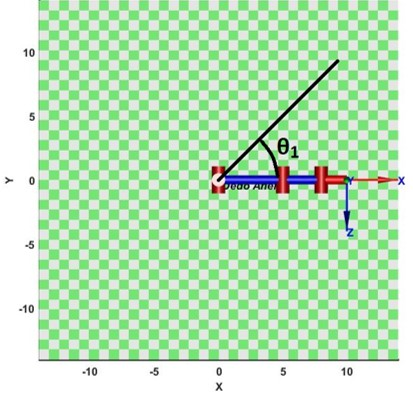
\includegraphics[width = 0.6\textwidth]{img/theta1.jpg}
\caption[Representação do ângulo $\theta_1$]{Representação do ângulo $\theta_1$}
\label{theta1}
\end{figure}

\begin{figure}[H]
\centering
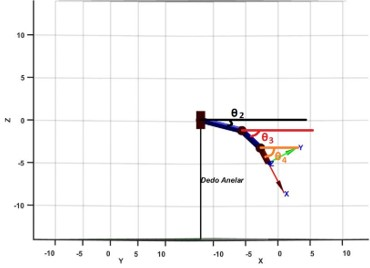
\includegraphics[width = 0.6\textwidth]{img/thetas.jpg}
\caption[Representação dos ângulos $\theta_2$, $\theta_3$ e $\theta_4$]{Representação dos ângulos $\theta_2$,$\theta_3$ e $\theta_4$}
\label{thetas}
\end{figure}

Correlacionando as juntas com as suas restrições, podemos destacar as restrições descritas para as juntas MP, PIP, DIP descritas na seção \ref{anatomia_mao}, e lembrando que o ângulo de flexão da junta DIP é relacionado ao ângulo da junta DIP como descrito em \ref{relacao_dip_pip}.
A partir dos parâmetros de DH é possível obter as matrizes de DH, onde pode-se obter as posições das juntas a partir dos ângulos em que as articulações estão dispostas. Mas é preciso determinar alguns parâmetros antes, como a distância entre as juntas, que, no dedo, seria representado pelo tamanho das falanges. Os parâmetros do tamanho das falanges foram obtidos através de medidas realizadas em algumas pessoas durante o projeto. Os parâmetros de tamanho de falange estão listados na tabela \ref{ParamResto} e as matrizes de DH para cada junta estão nas equações \ref{matriz_junta1}, \ref{matriz_junta2}, \ref{matriz_junta3} e \ref{matriz_junta4}.
As matrizes de cada junta em relação a junta anterior estão dispostas em \ref{junta1}, \ref{junta2}, \ref{junta3} e \ref{junta4} 
\begin{align}
A_1=
\begin{bmatrix}
cos_1 & 0 & -sen_1 & 0\\
sen_1 & 0 & cos_1 & 0\\
0 & -1 & 0 & 0\\
0 & 0 & 0 & 1\\
\end{bmatrix} \label{junta1}\\
A_2=
\begin{bmatrix}
cos_2 & -sen_2 & 0 & l1*cos_2\\
sen_2 & cos_2 & 0 & l1*sen_2\\
0 & 0 & 1 & 0\\
0 & 0 & 0 & 1\\
\end{bmatrix}  \label{junta2} \\
A_3=
\begin{bmatrix}
cos_3 & -sen_3 & 0 & l2*cos_3\\
sen_3 & cos_3 & 0 & l2*sen_3\\
0 & 0 & 1 & 0\\
0 & 0 & 0 & 1\\
\end{bmatrix}  \label{junta3} \\
A_4=
\begin{bmatrix}
cos_4 & -sen_4 & 0 & l3*cos_4\\
sen_4 & cos_4 & 0 & l3*sen_4\\
0 & 0 & 1 & 0\\
0 & 0 & 0 & 1\\
\end{bmatrix} \label{junta4}
\end{align}

\begin{align}
A_{MP_{AA}}= A_1 \label{matriz_junta1}\\
A_{MP_{F}}= A_1 * A_2 \label{matriz_junta2} \\
A_{PIP_{F}}= A_1 * A_2 * A_3 \label{matriz_junta3} \\
A_{DIP_{F}}= A_1 * A_2 * A_3 * A_4 \label{matriz_junta4}
\end{align}

Sendo $cos_i$ e $sen_i$ as representações de $cos(\theta_i)$ e $sen(\theta_i)$, e lembrando que $\theta_4 = \frac{2}{3}\theta_3$.

Com as tabelas é possível obter o posicionamento da junta em qualquer instante de tempo, dado os ângulos das juntas, estes provenientes do sistema de forças introduzido pelo modelo de Hill \cite{hill1938heat}. O posicionamento das juntas na tabela é descrito pela última coluna, onde as posições em cada eixo cartesiano é representado em uma linha, na linha 1 fica o valor do eixo x, na linha 2 fica o valor do eixo y e na linha 3 fica o valor do eixo z.

Para validar a restrição da angulação entre as juntas PIP e DIP foi simulado a resposta do dedo ao mover apenas a junta DIP, com uma entrada mostrada na figura \ref{ang_sim_pip}. A resposta para esta entrada está na figura \ref{sim_pip}, e é possível notar como a ângulação da junta DIP se move conforme a junta PIP porém com valores menores. Os ângulos para esta simulação foram retirados de medição empírica sobre dedos de algumas pessoas.

\begin{figure}[H]
\centering
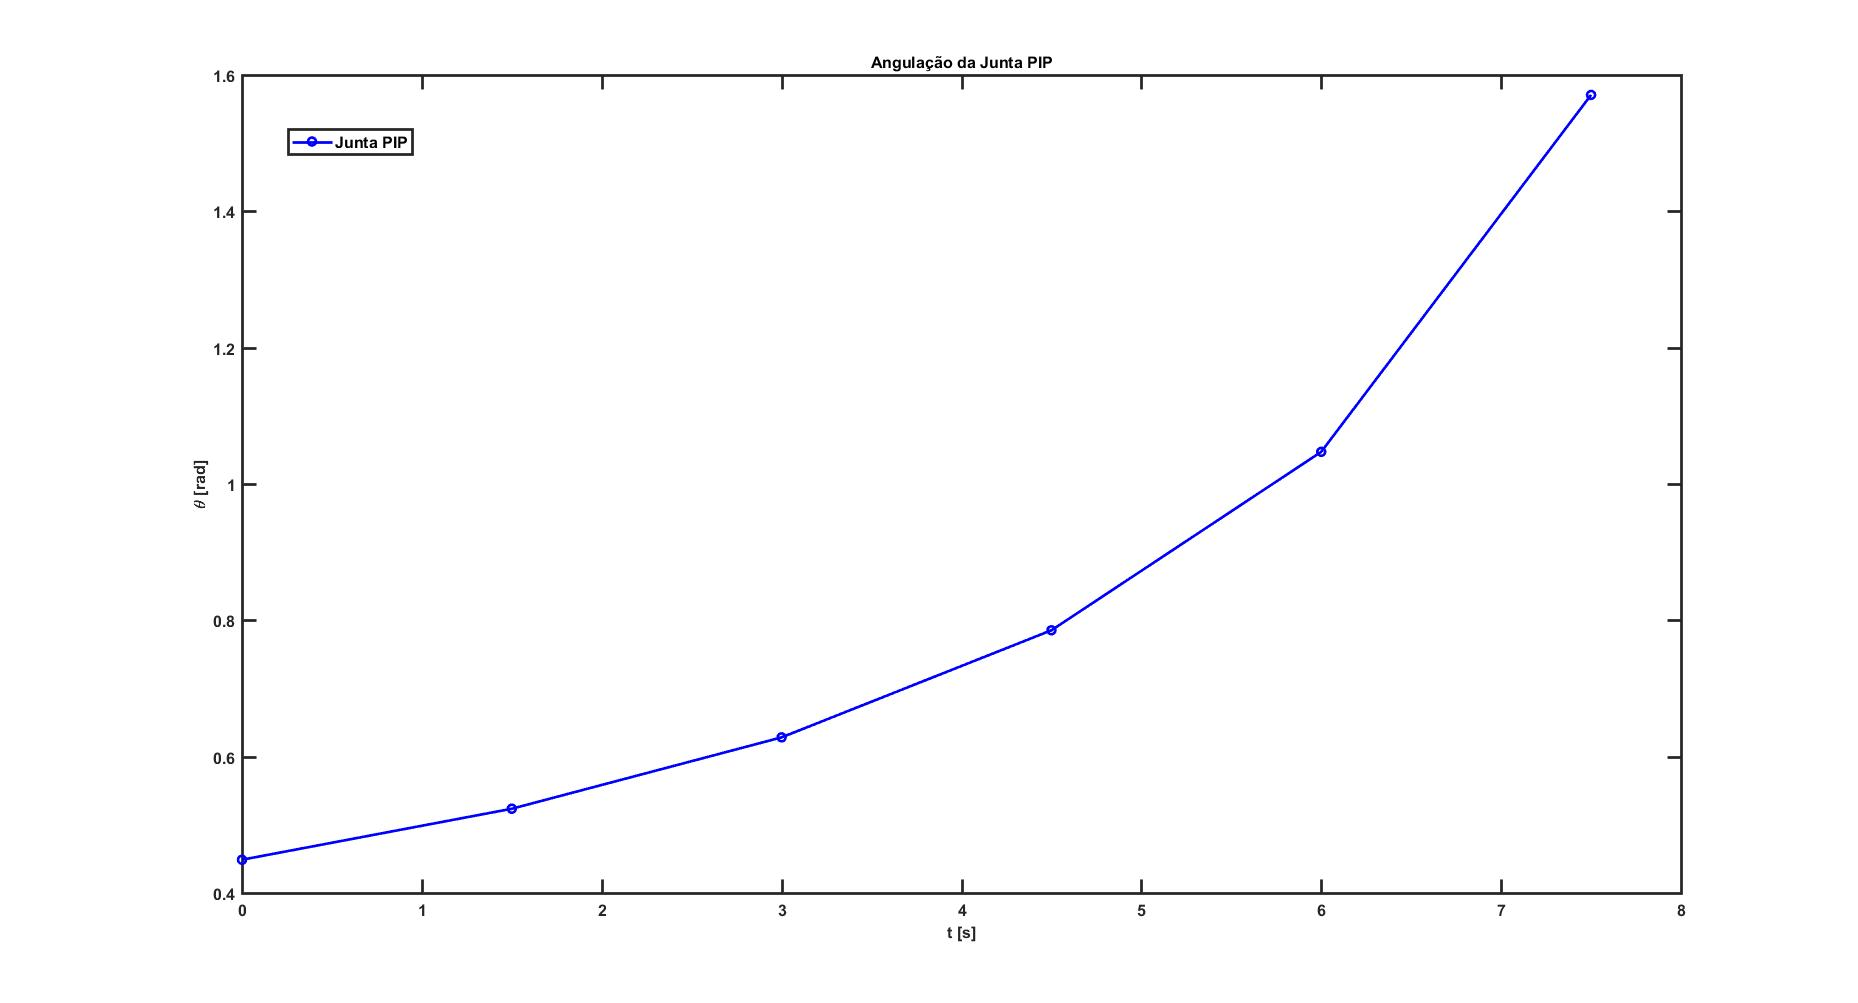
\includegraphics[width = 1\textwidth]{img/angulacao_pip.jpg}
\caption[Ângulos de simulação de entrada para a junta PIP]{Ângulos de simulação de entrada para a junta PIP}
\label{ang_sim_pip}
\end{figure}

\begin{figure}[H]
\centering
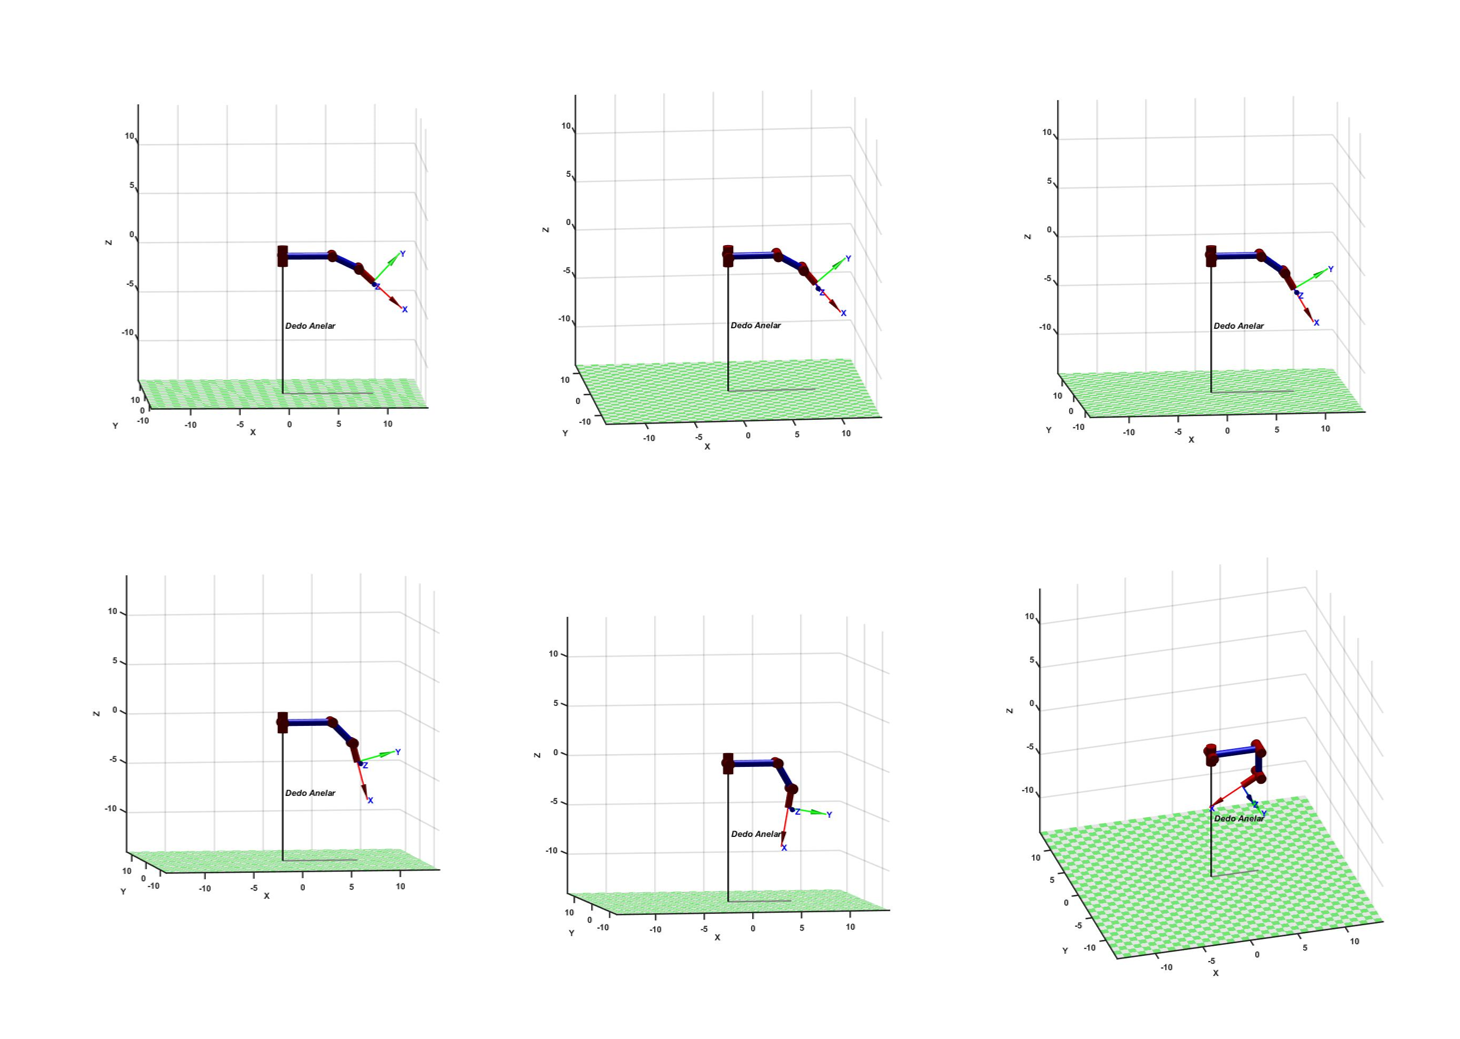
\includegraphics[width = 1\textwidth]{img/simpip.png}
\caption[Simulação de entrada para a junta PIP]{Simulação de entrada para a junta PIP}
\label{sim_pip}
\end{figure}

\begin{figure}[H]
\centering
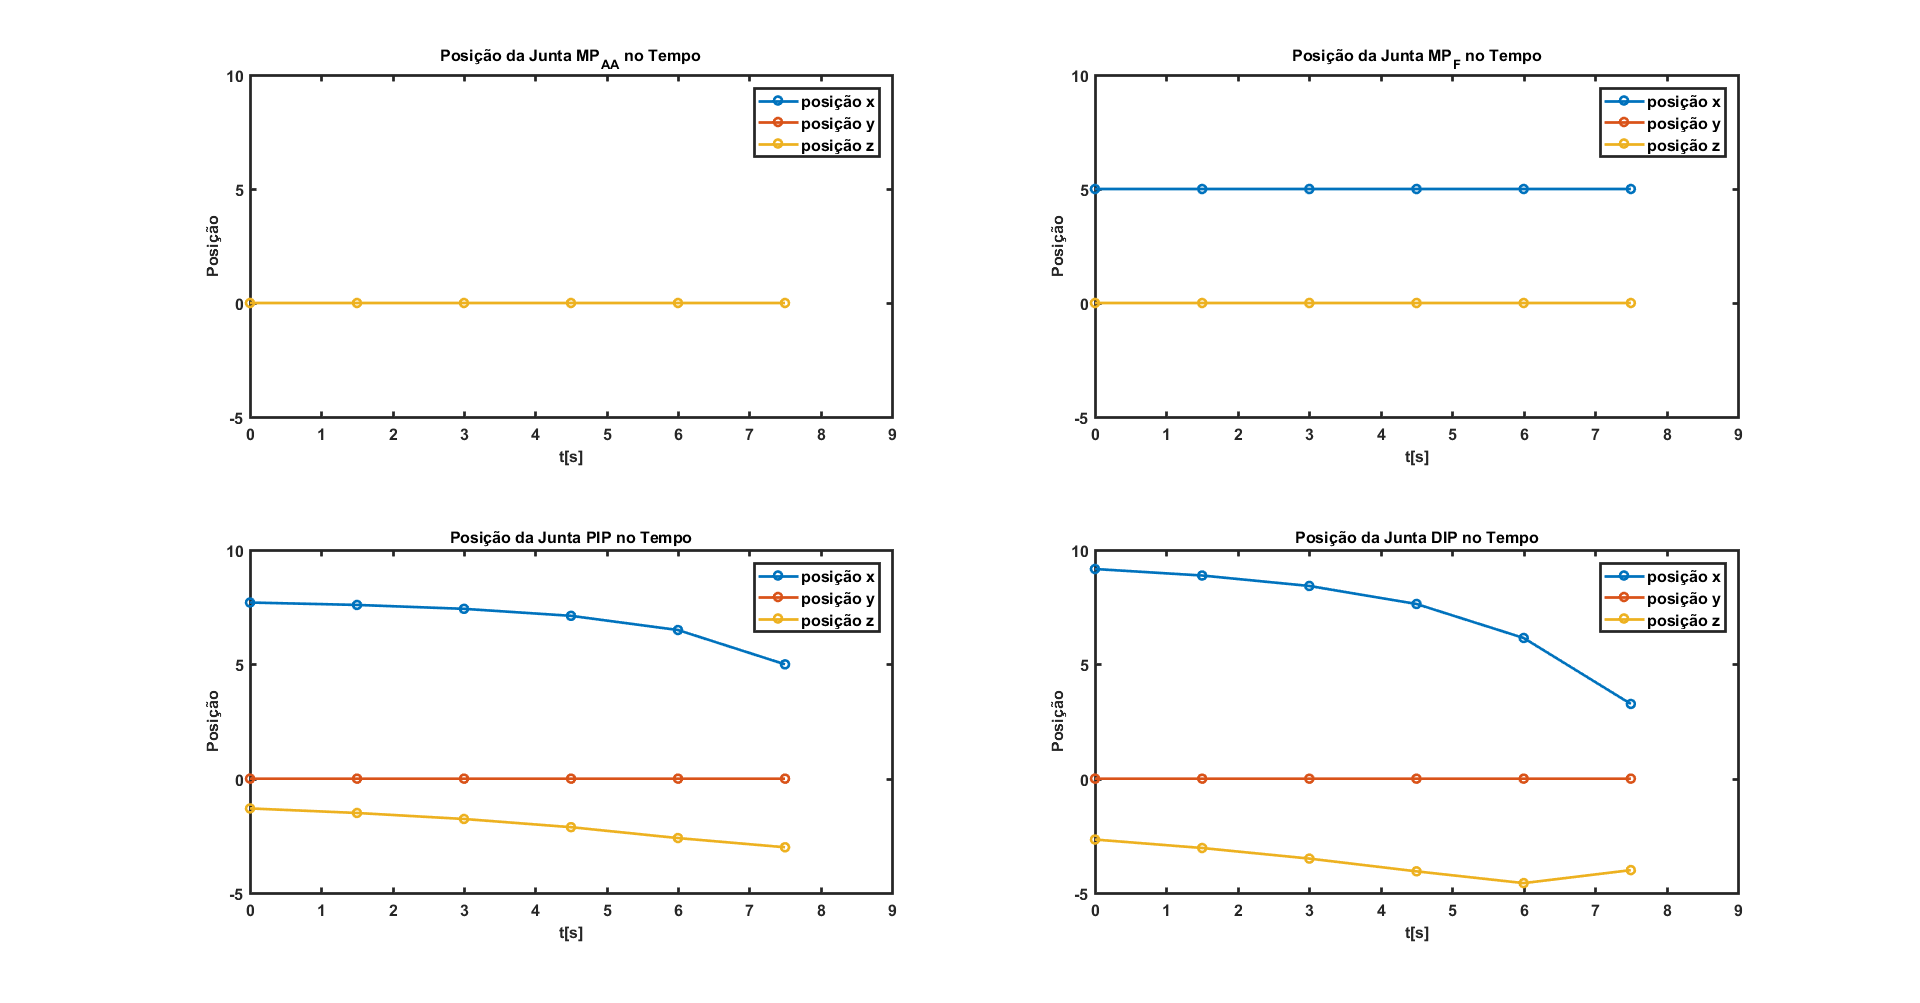
\includegraphics[width = 1\textwidth]{img/posicoes_pip.png}
\caption[Posições das Juntas em Função do Tempo - Simulação de entrada para a junta PIP]{Posições das Juntas em Função do Tempo - Simulação de entrada para a junta PIP}
\end{figure}

O mesmo é feito para a junta MP, onde foram aplicados os ângulos de entrada para os músculos de flexão e abudção/adução descritos na figura \ref{ang_sim_mp}. A resposta para esta entrada está na figura \ref{sim_mp}, onde é possível notar a movimentação das duas juntas e como o dedo se comporta quando estes músculos estão sobre força. Lembra-se que o ângulo de adução/abdução da junta MP é limitado em um range de $-15^\circ$ à $15^\circ$, por isso sua variação angular é pequena perto do ângulo de flexão. Os ângulos para esta simulação foram retirados de medição empírica sobre dedos de algumas pessoas.

\begin{figure}[H]
\centering
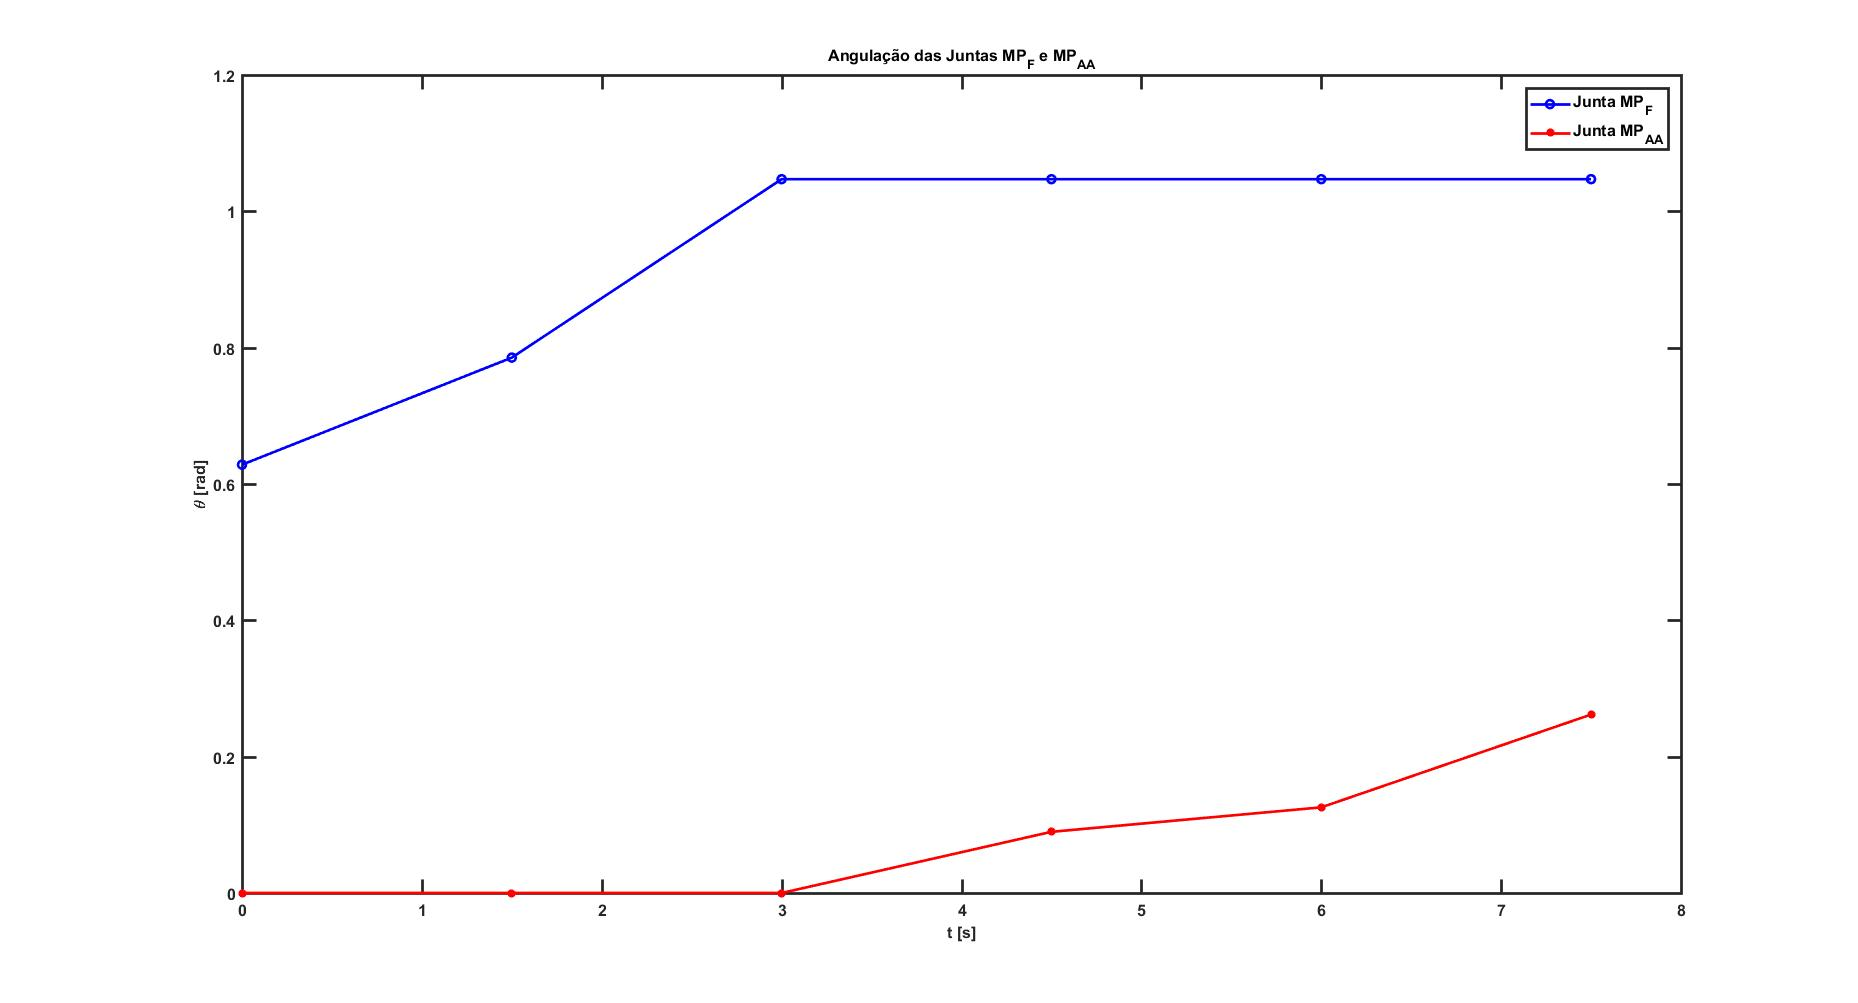
\includegraphics[width = 1\textwidth]{img/angulacao_mp.jpg}
\caption[Ângulos de simulação de entrada para a junta MP]{Ângulos de simulação de entrada para a junta MP}
\label{ang_sim_mp}
\end{figure}

\begin{figure}[H]
\centering
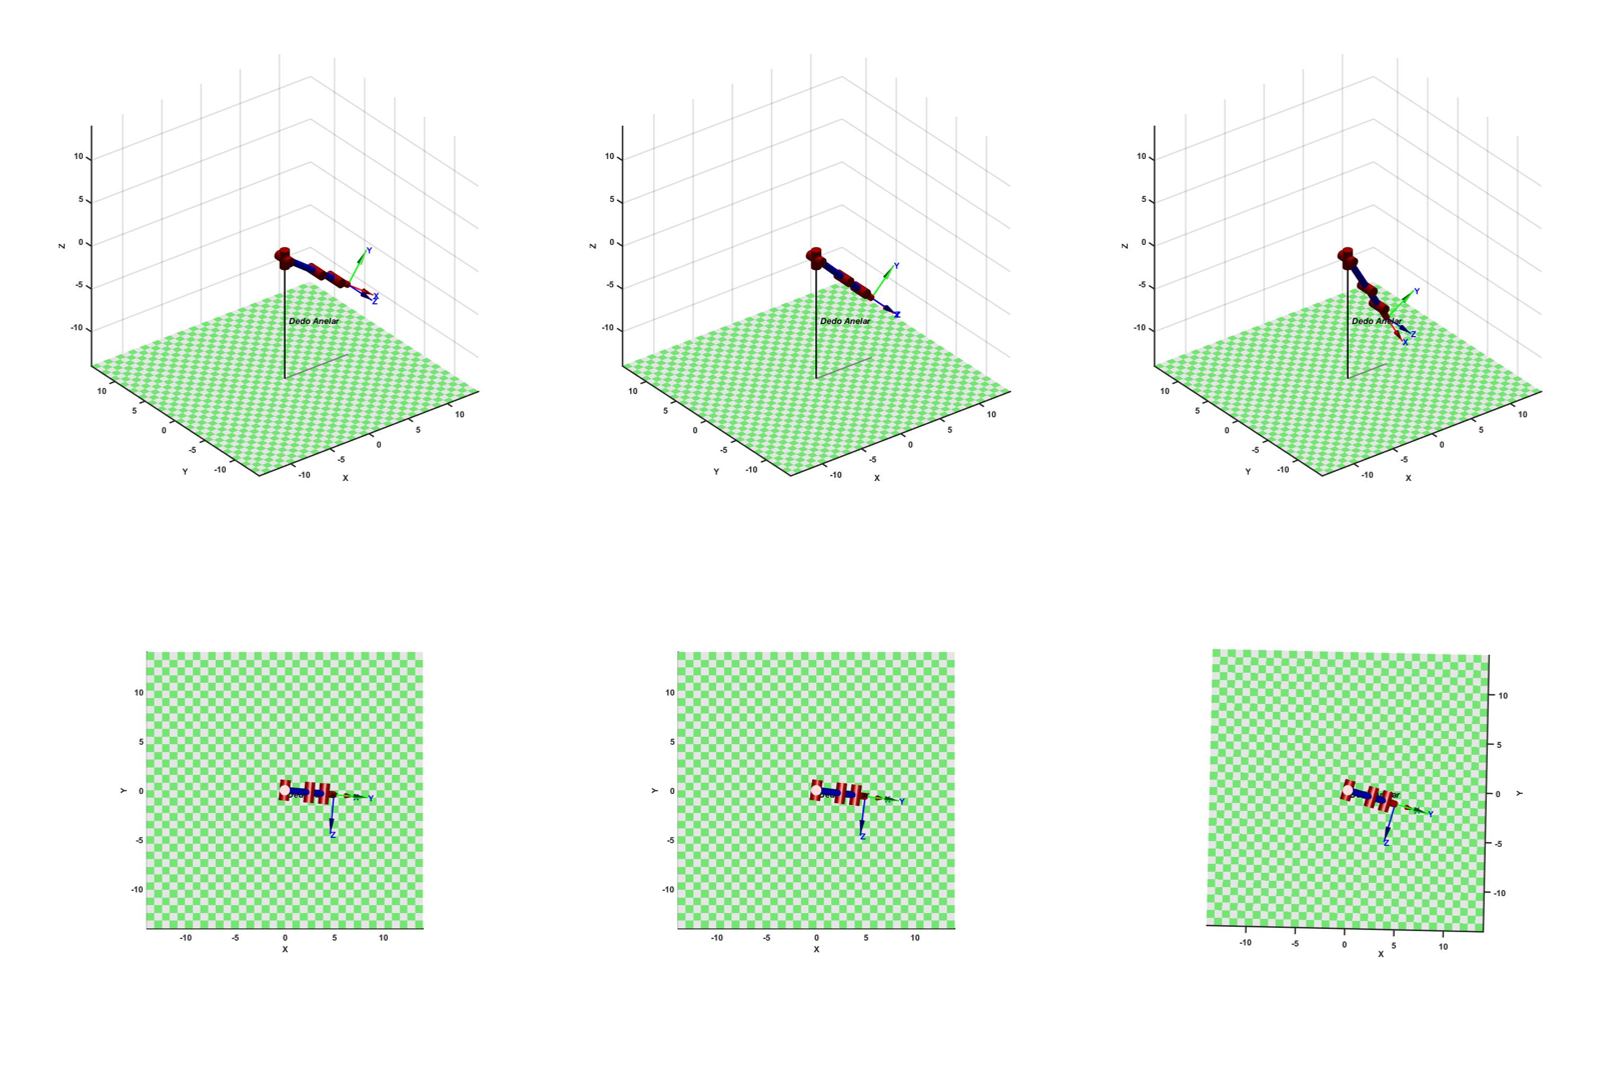
\includegraphics[width = 1\textwidth]{img/simmp.png}
\caption[Simulação de entrada para a junta MP]{Simulação de entrada para a junta MP}
\label{sim_mp}
\end{figure}

\begin{figure}[H]
\centering
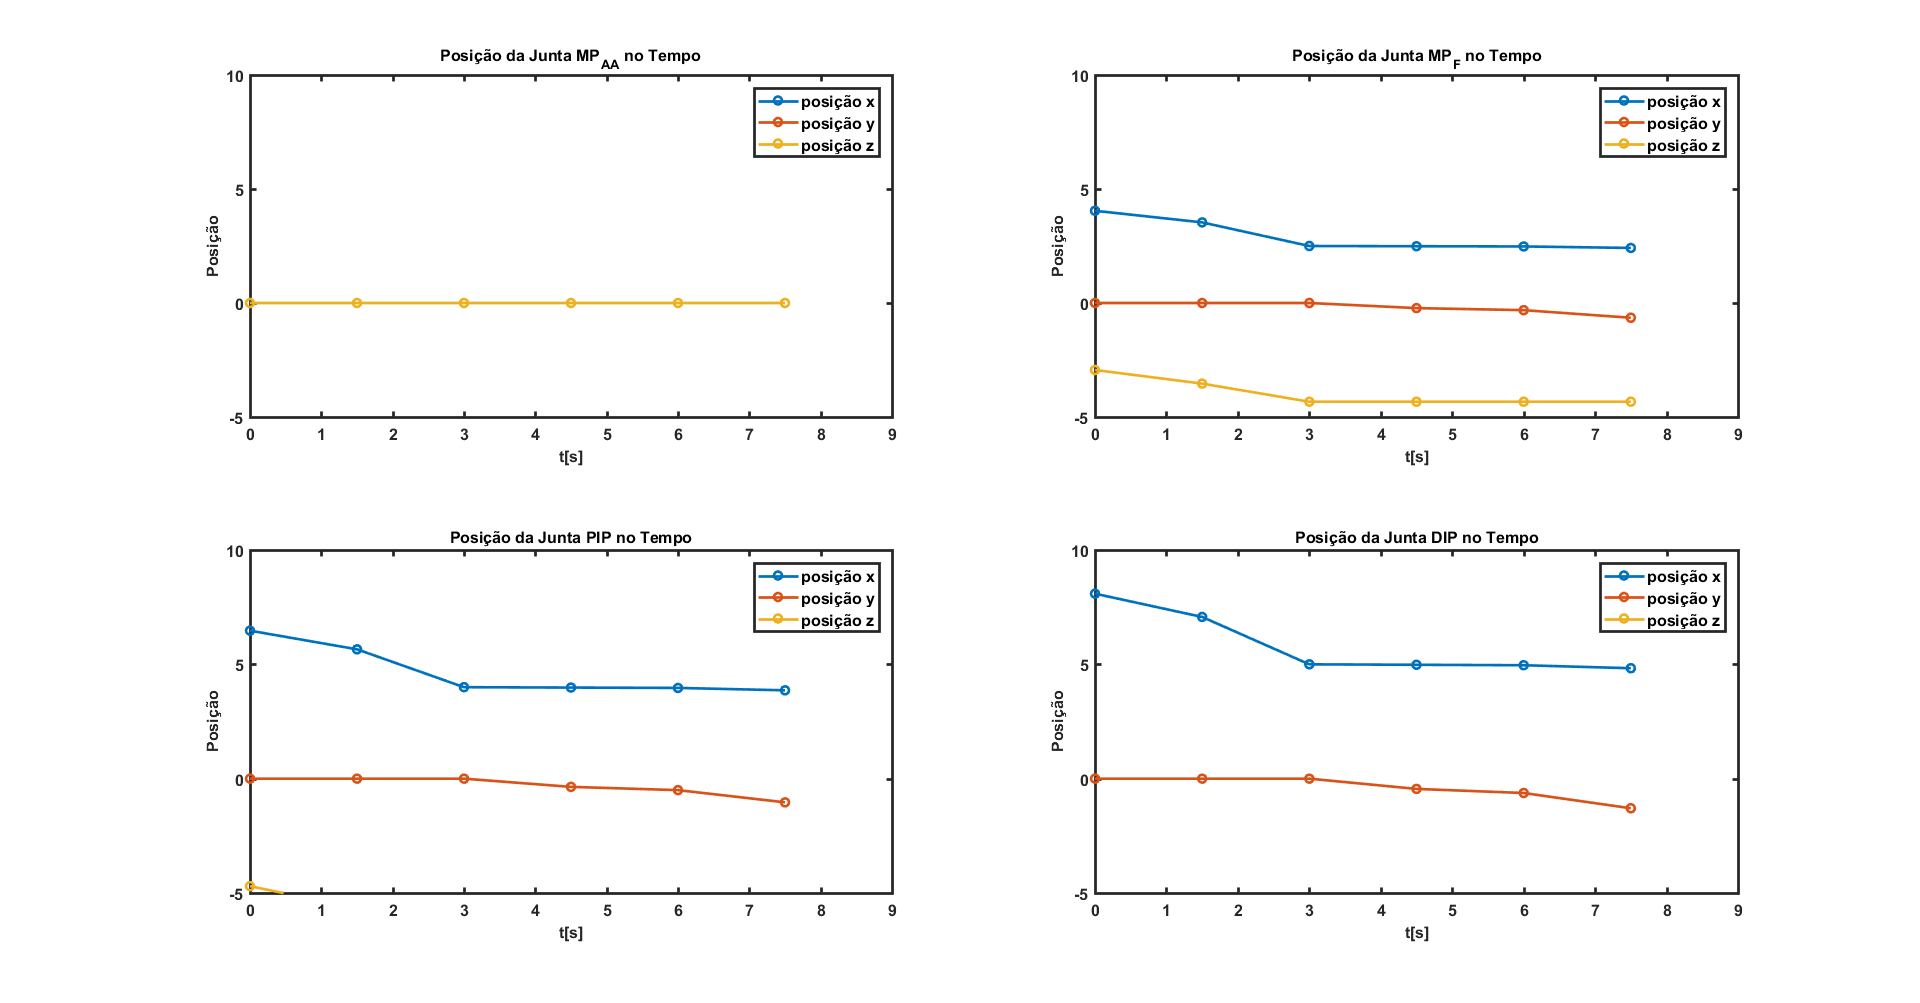
\includegraphics[width = 1\textwidth]{img/posicoes_mp.png}
\caption[Posições das Juntas em Função do Tempo - Simulação de entrada para a junta MP]{Posições das Juntas em Função do Tempo - Simulação de entrada para a junta MP}
\end{figure}

E por fim, uma simulação de todas as juntas estimuladas, demonstrando que as matrizes de DH representam bem o movimento de um dedo para as entradas da figura \ref{ang_sim_DH}. A figura \ref{sim_DH} representa a movimentação do dedo quando a entrada é a da figura \ref{ang_sim_DH}.

\begin{figure}[H]
\centering
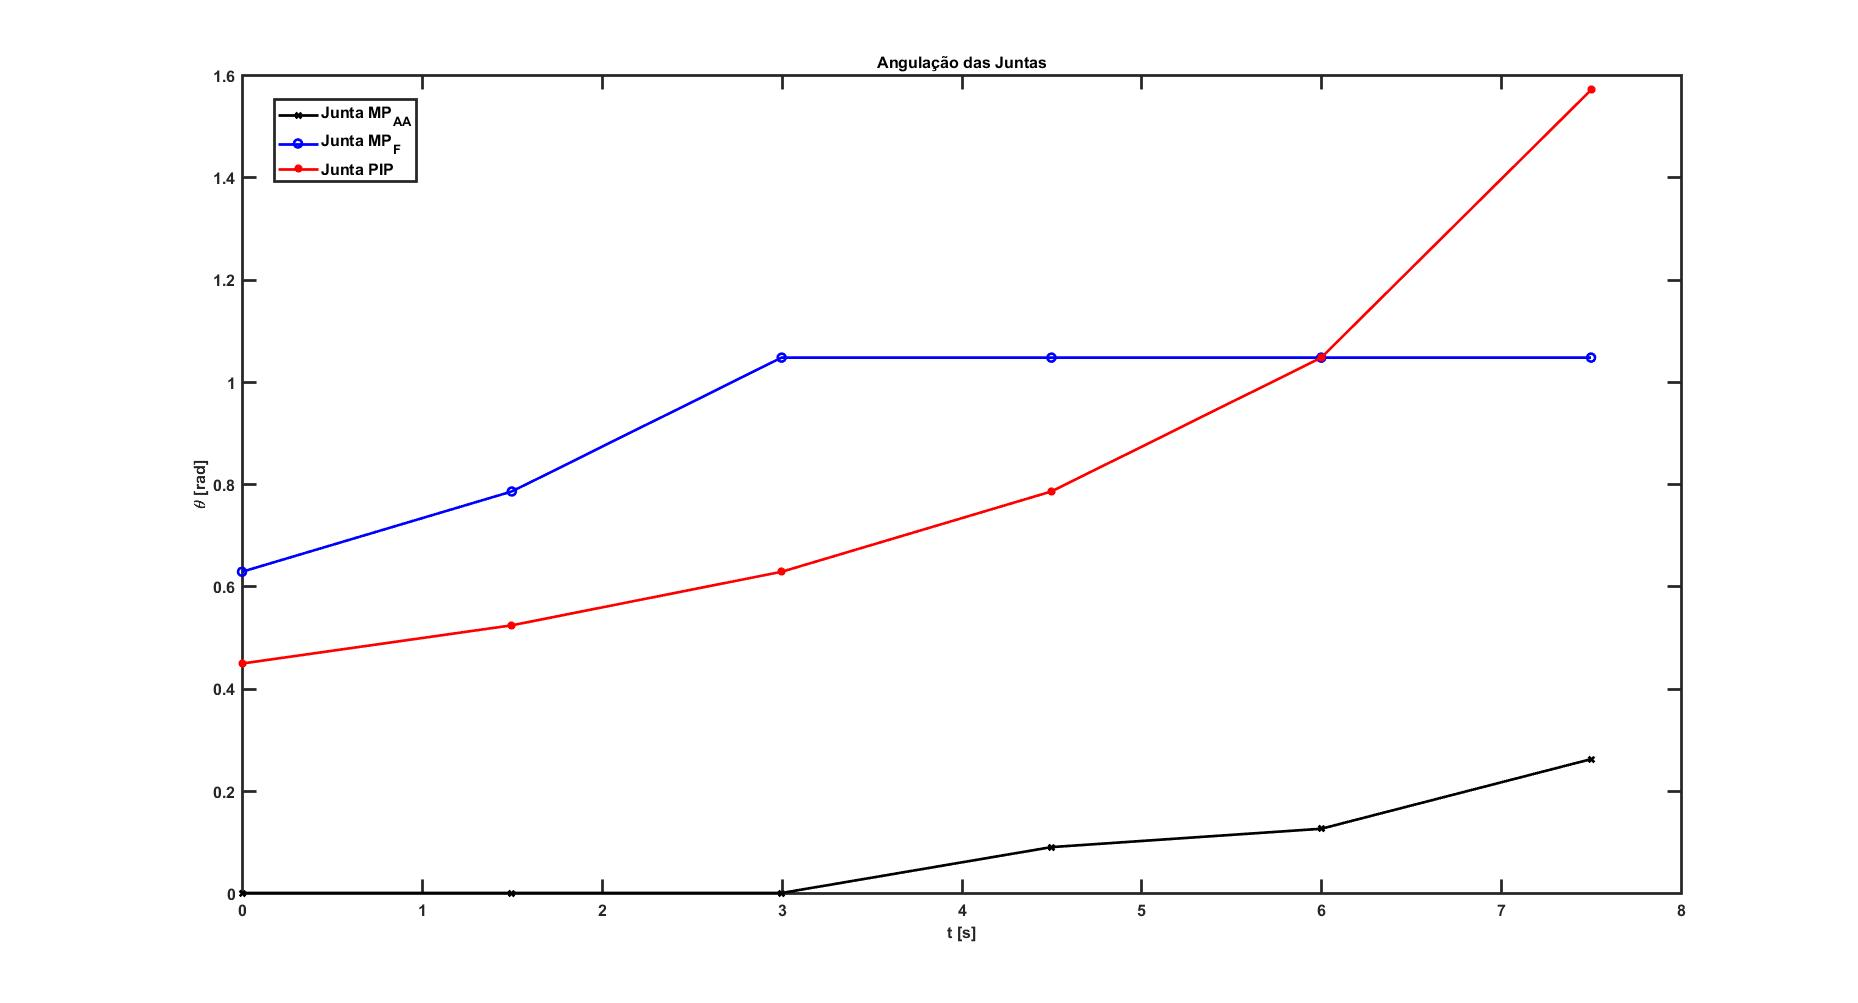
\includegraphics[width = 1\textwidth]{img/angulacao_tudo.jpg}
\caption[Ângulos de simulação de entrada para todas as juntas]{Ângulos de simulação de entrada para todas as juntas}
\label{ang_sim_DH}
\end{figure}

\begin{figure}[H]
\centering
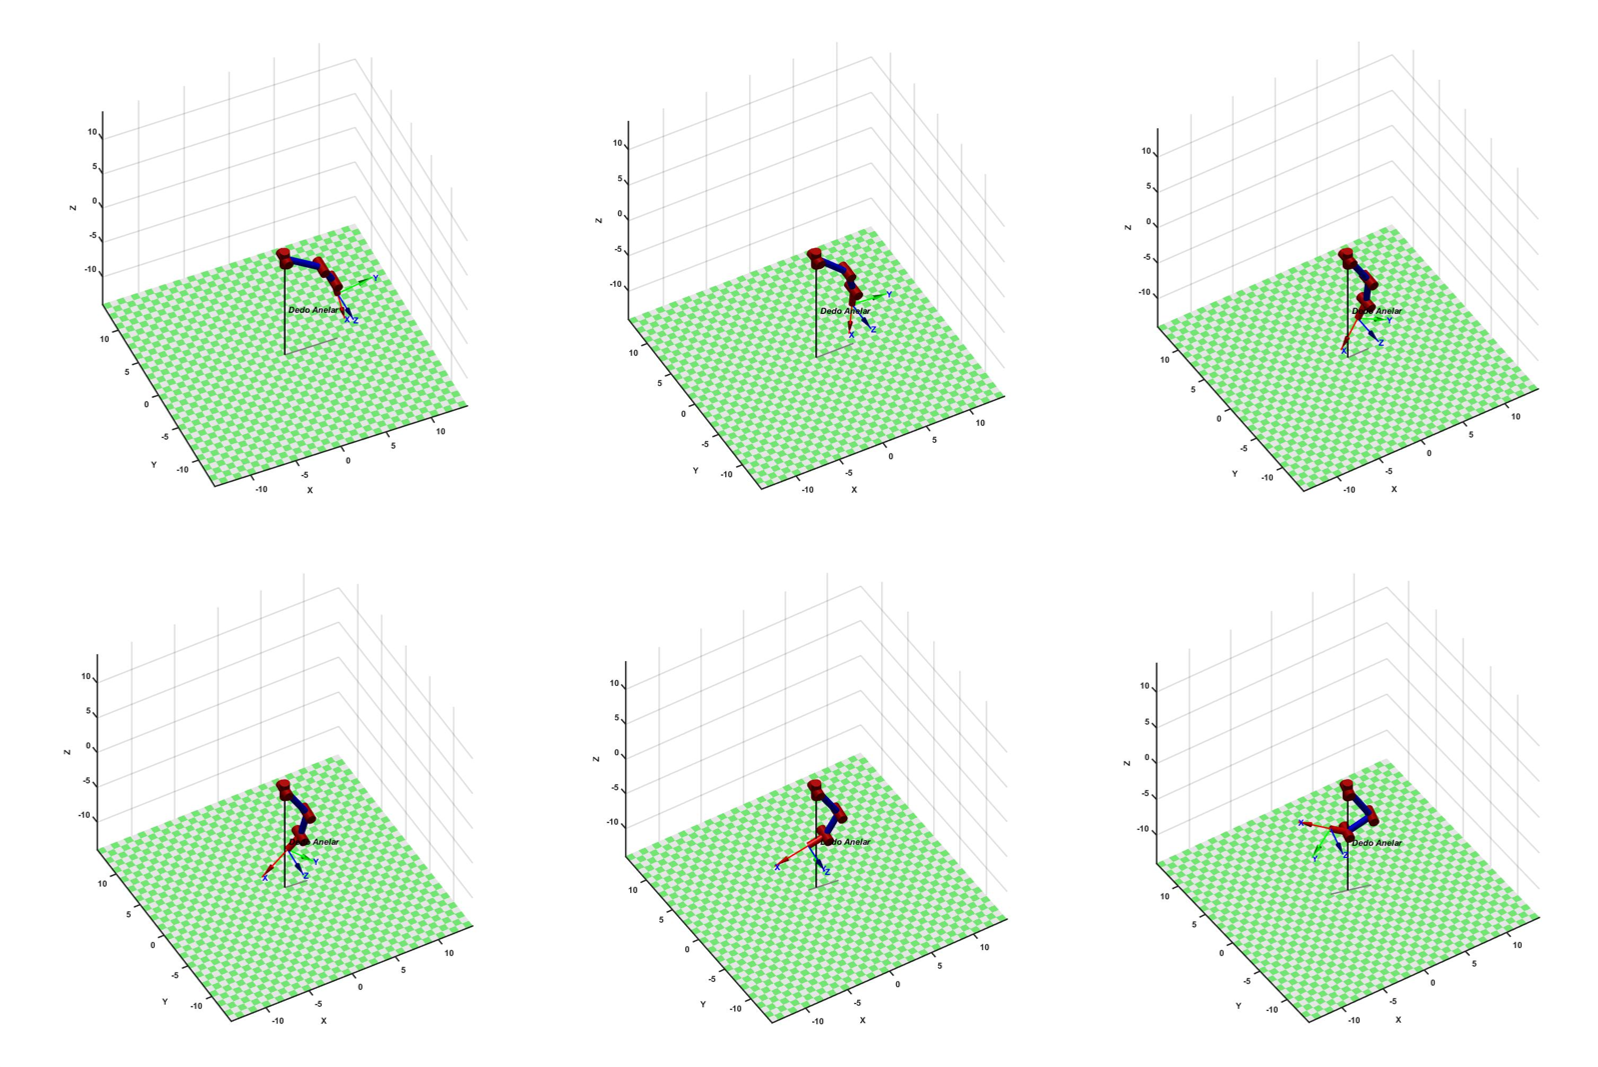
\includegraphics[width = 1\textwidth]{img/sim_total.png}
\caption[Simulação de entrada para todas as juntas]{Simulação de entrada para todas as juntas}
\label{sim_DH}
\end{figure}

\begin{figure}[H]
\centering
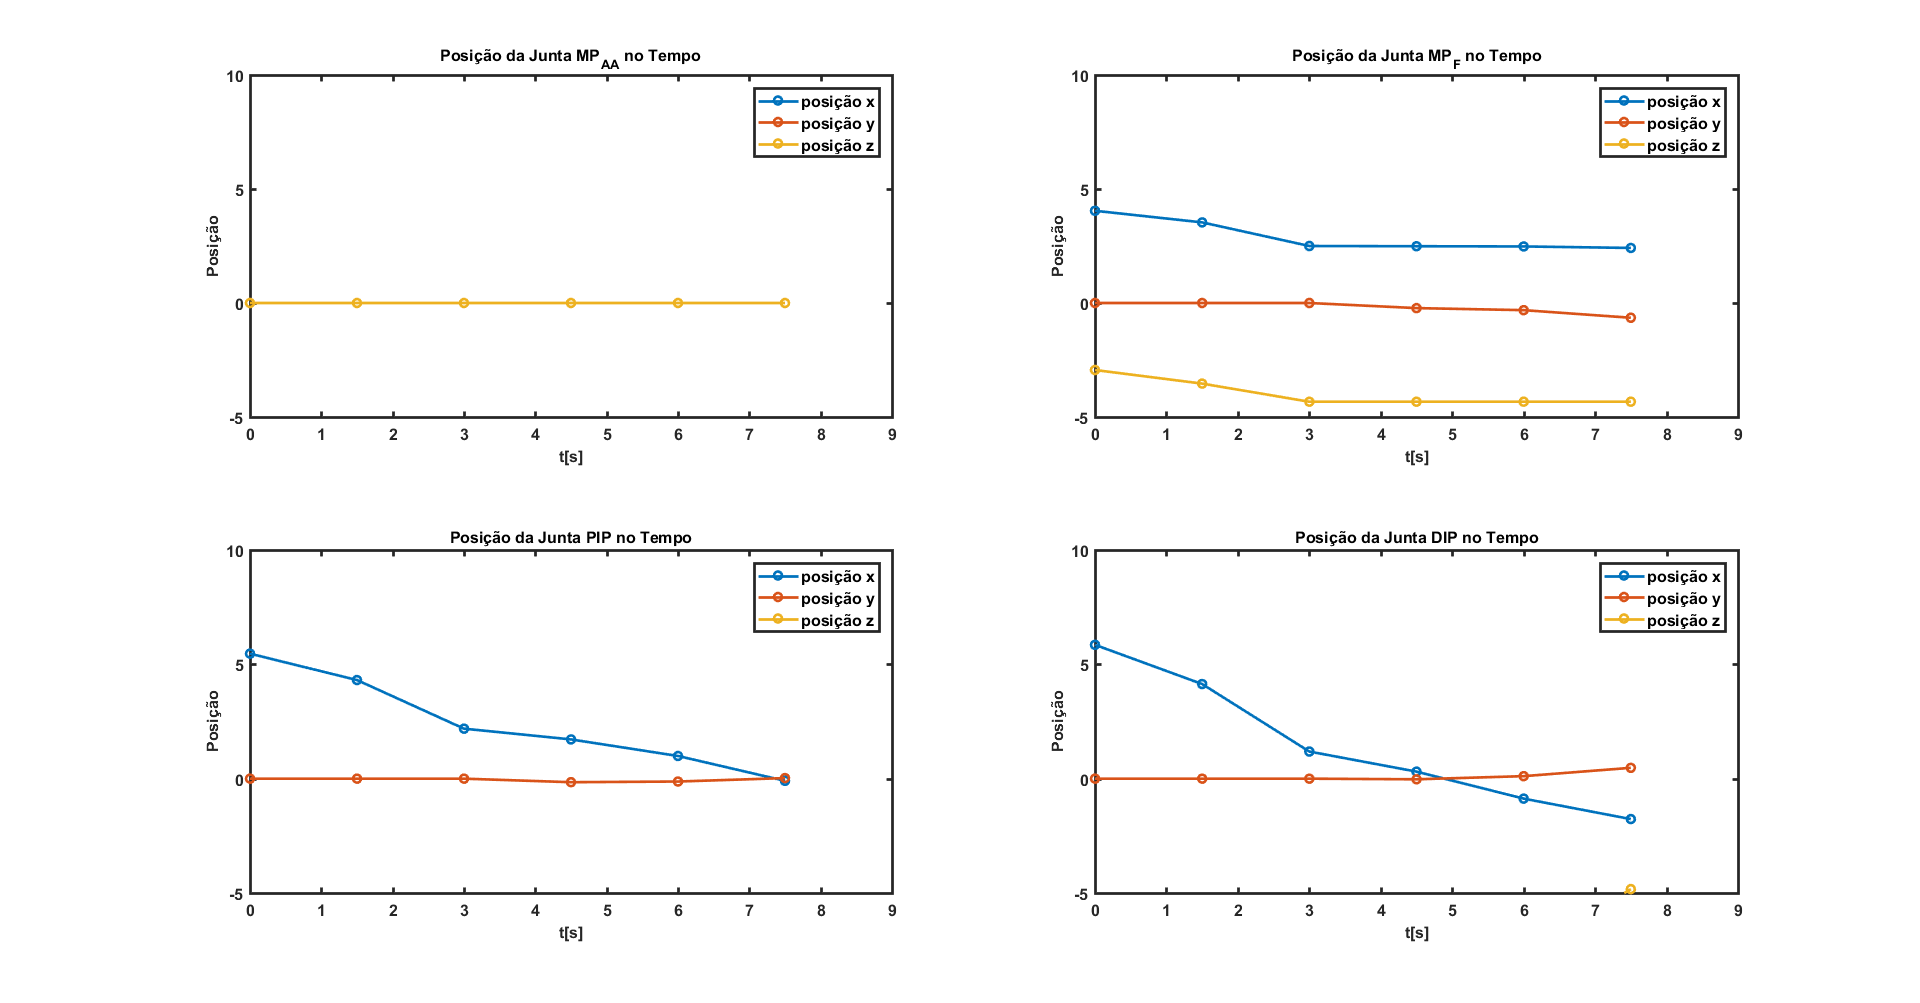
\includegraphics[width = 1\textwidth]{img/todas_juntas.png}
\caption[Posições das Juntas em Função do Tempo - Simulação de entrada para as juntas]{Posições das Juntas em Função do Tempo - Simulação de entrada para as juntas}
\label{ang_sim_DH}
\end{figure}

\section{Modelagem da Ativação Muscular}
\label{resultado_ativacao}
Como explicado em \cite{zajac1989muscle} existem relações entre o nível de ativação muscular e o ângulo das articulações. Estas relações podem ser modeladas como foi proposto por \cite{feng1999surface} e mostrado na seção \ref{forcas_modelo_simplificado} é possível criar um modelo no \textit{SIMULINK} capaz de aproximar estas resoluções. O objetivo desta simulação é colher os dados de saída do modelo feito no \textit{SIMULINK} e compará-los aos de outros estudos como de \cite{zajac1989muscle}, \cite{rosen1999performances} e \cite{feng1999surface}. Para esta análise foi necessário definir algumas constantes empíricas para o funcionamento do modelo, como o MJG (da seção \ref{forcas_modelo_simplificado}) e os ângulos de repouso das juntas. Naturalmente, como evidenciado em \cite{lin2000modeling} os dedos da mão não ficam totalmente alinhados com o resto da mão quando em repouso, isso justifica as saídas de angulação da junta que não partem do $0^\circ$. 

Para este estudo o valor de MJG para as diferentes falanges está disposto na tabela \ref{MJG_tabela}, os diferentes valores foram obtidos de forma empírica enquanto se fazia o estudo, já que não foram encontrados valores conclusivos na literatura. O valor da geometria das articulações varia conforme as falanges devido, justamente, a geometria de cada falange, seu comprimento e circunferência são fatores que demonstram as diferenças neste parâmetro.

\begin{table}[H]
\centering
\caption{Tabela de Valores para MJG}
\label{MJG_tabela}
\begin{tabular}{|c|c|c|}
	\hline
    Falange & Valor de MJG (m) \\ \hline
    Falange próxima & 20 \\ \hline
    Falange média & 10 \\ \hline
    Falange distal & 5 \\
	\hline
\end{tabular}
\end{table}

Este valor, como proposto por \cite{feng1999surface} é o ganho que converte os torques exercidos pelos músculos em ângulos, velocidades e acelerações nas articulações.

Nesta simulação são feitos os movimentos de flexão e extensão de um músculo. Como este é um modelo normalizado, as respostas esperadas para estes movimentos podem ser aplicadas para os outros músculos dos dedos sem perda de coerência dos dados. Portanto esta simulação é feita sobre a falange próxima de um dedo da mão. Primeiramente, é executada a ação de flexionar o músculo colocando como entrada um nível de ativação máximo igual a 1, já que o modelo é normalizado. Assim que a ativação do movimento de flexão cessa, se inicia a ativação do músculo de extensão de mesma intensidade. O uso destes dois músculos foi previsto na seção \ref{integracao_validacao}, e ambas as forças dos músculos são dadas como positivas e então o sinal é alterado conforme o músculo atua como avanço ou recuo.

Os sinais utilizados para realizar os movimentos de flexão e extensão estão ilustrados na figura \ref{ativacao_musculos}.

\begin{figure}[H]
\centering
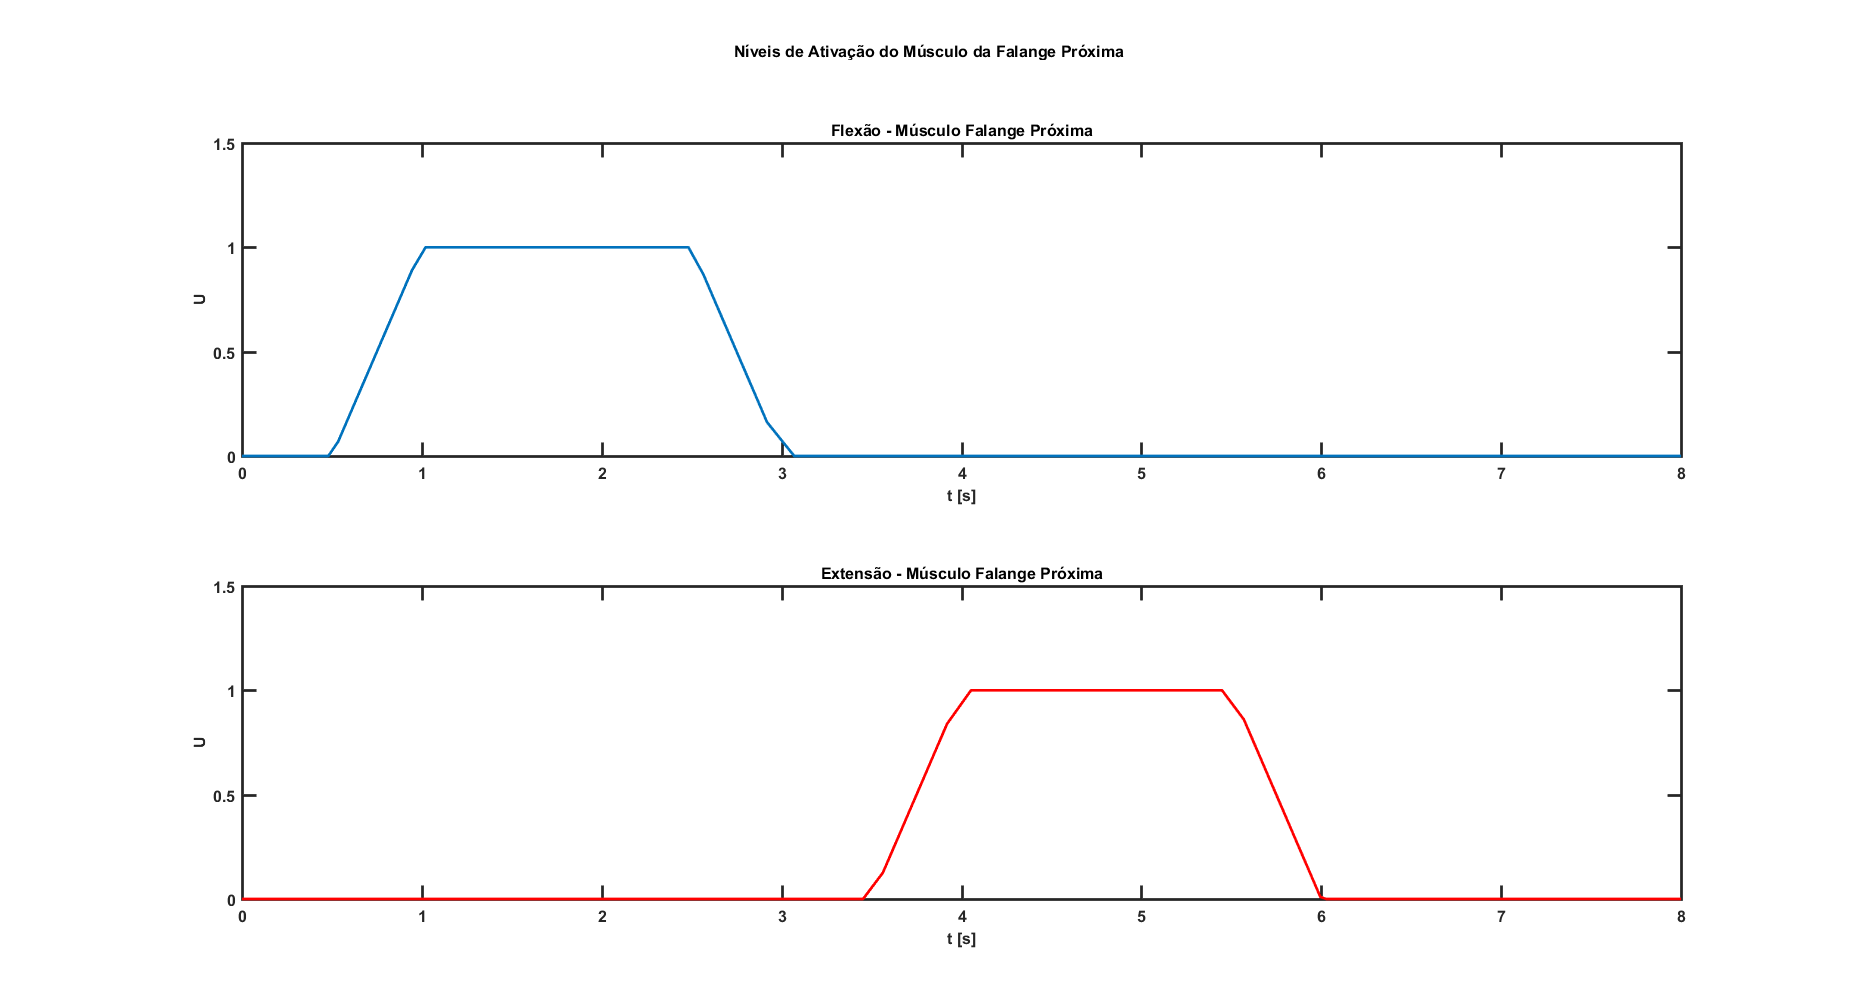
\includegraphics[width = 1\textwidth]{img/niveis_ativacao.png}
\caption[Níveis de Ativação para Flexão e Extensão para os Músculos de uma Falange Próxima]{Níveis de Ativação para Flexão e Extensão para os Músculos de uma Falange Próxima}
\label{ativacao_musculos}
\end{figure}

Ao excitar o músculo de flexão com um nível de ativação $U=1$ espera-se uma resposta condizente com as propostas por \cite{rosen1999performances}, onde a força do elemento CE depende do nível de atuação e a força do elemento PE não depende do nível de atuação, e sim do comprimento do músculo \cite{zajac1989muscle}. De início é feito a simulação como se só houvesse o movimento de flexão do músculo, para analisar qual é a resposta dos elementos de força do músculo e como seria a saída do modelo, em velocidade e ângulo. A figura \ref{sim_flexao} mostra o resultado da simulação de flexão pura. É possível notar que o elemento CE do músculo de flexão é ativado conforme o nível de ativação, e uma vez que este cessa o elemento CE não apresenta mais força, porém o elemento PE que possui sua saída de força atrelada ao comprimento do movimento, continua apresentando uma saída de força, justamente por que não houve uma extensão do músculo após a flexão, ou seja, o músculo continua "tensionado". É possível notar o mesmo comportamento no comprimento do músculo e na angulação de saída da junta, eles permanecem estáticos mesmo após o nível de atuação do movimento de flexão ter acabado.

\begin{figure}[H]
\centering
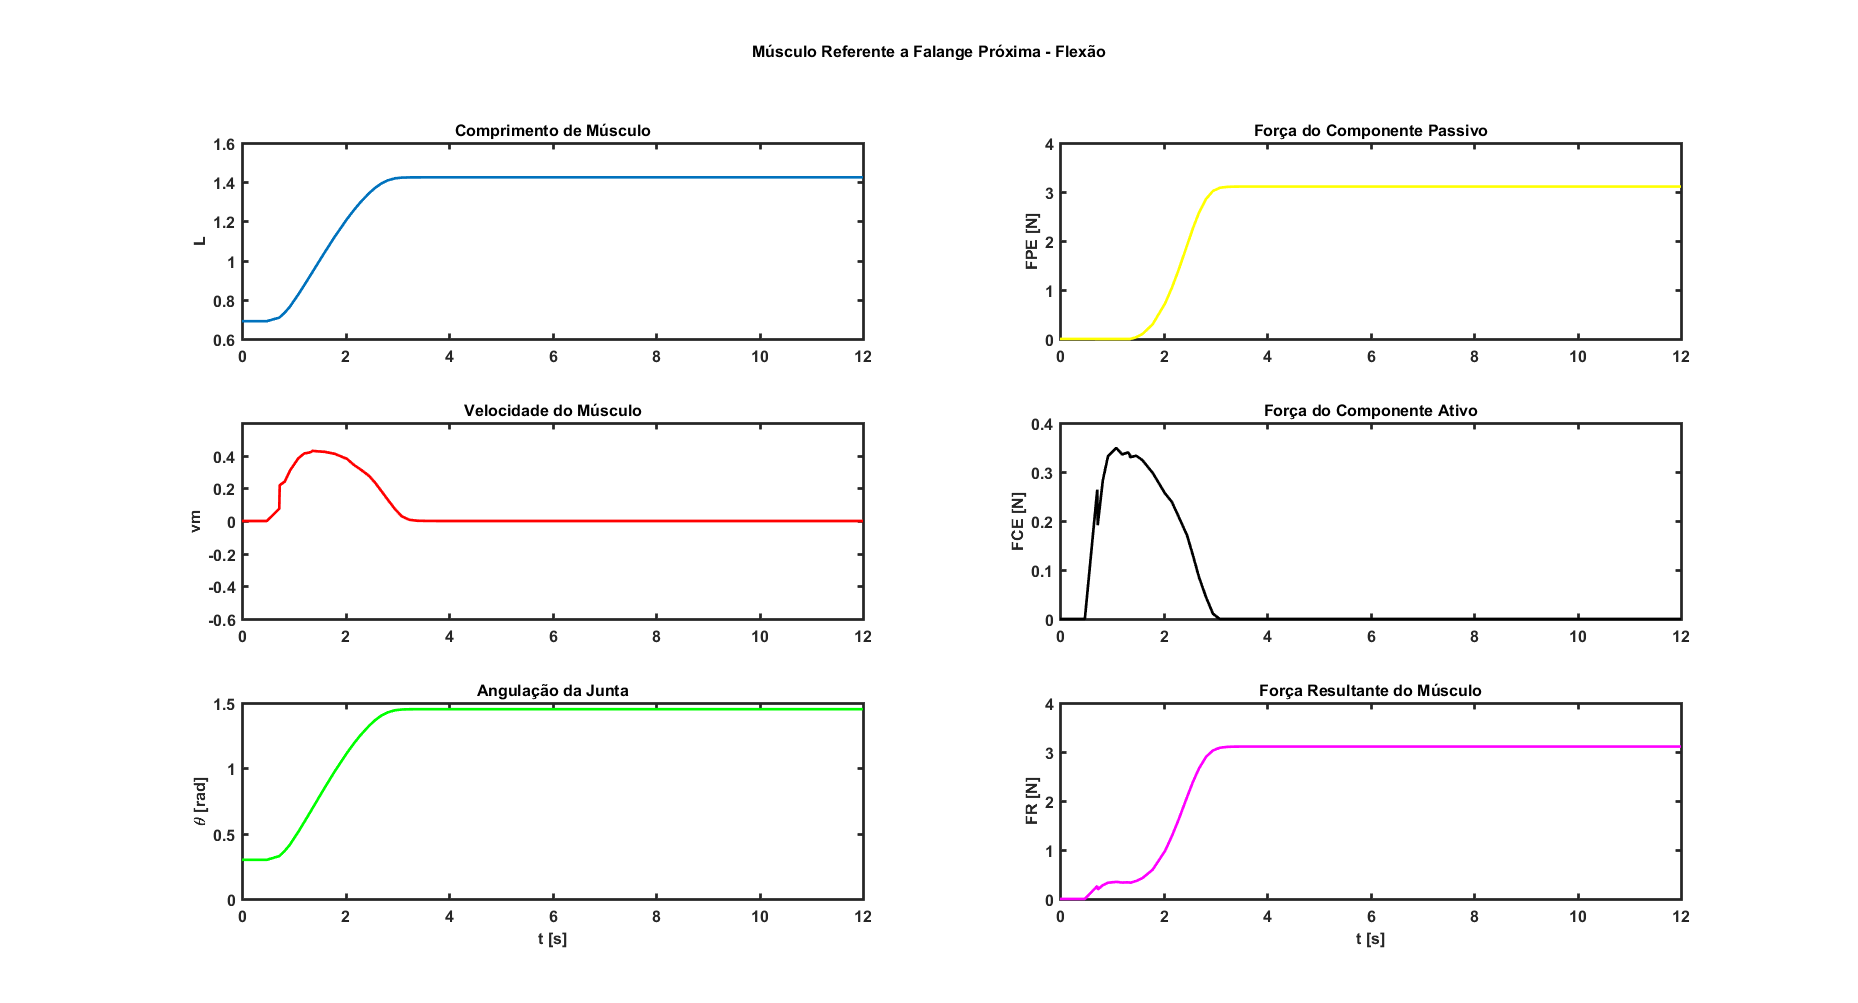
\includegraphics[width = 1\textwidth]{img/flexao.png}
\caption[Resposta ao Movimento de Flexão para uma Falange Próxima]{Resposta ao Movimento de Flexão para uma Falange Próxima}
\label{sim_flexao}
\end{figure}

Ao mesmo passo que o nível de ativação foi utilizado para uma flexão pura, é feito uma extensão no músculo assim que a flexão acaba. Com isso os níveis de atuação utilizados passam a ser exatamente os dois da figura \ref{ativacao_musculos}, já que antes era somente o primeiro destes. A resposta para um movimento de flexão e então extensão está ilustrado na figura \ref{sim_flexao_extensao}. Nesta resposta é possível notar que o movimento de extensão faz com que o comprimento do músculo volte a 0 e assim o elemento PE passa a não apresentar mais uma resposta de força. Sendo assim os outros parâmetros de saída do modelo acompanham e apresentam uma curva plausível com o movimento físico dos músculos.

\begin{figure}[H]
\centering
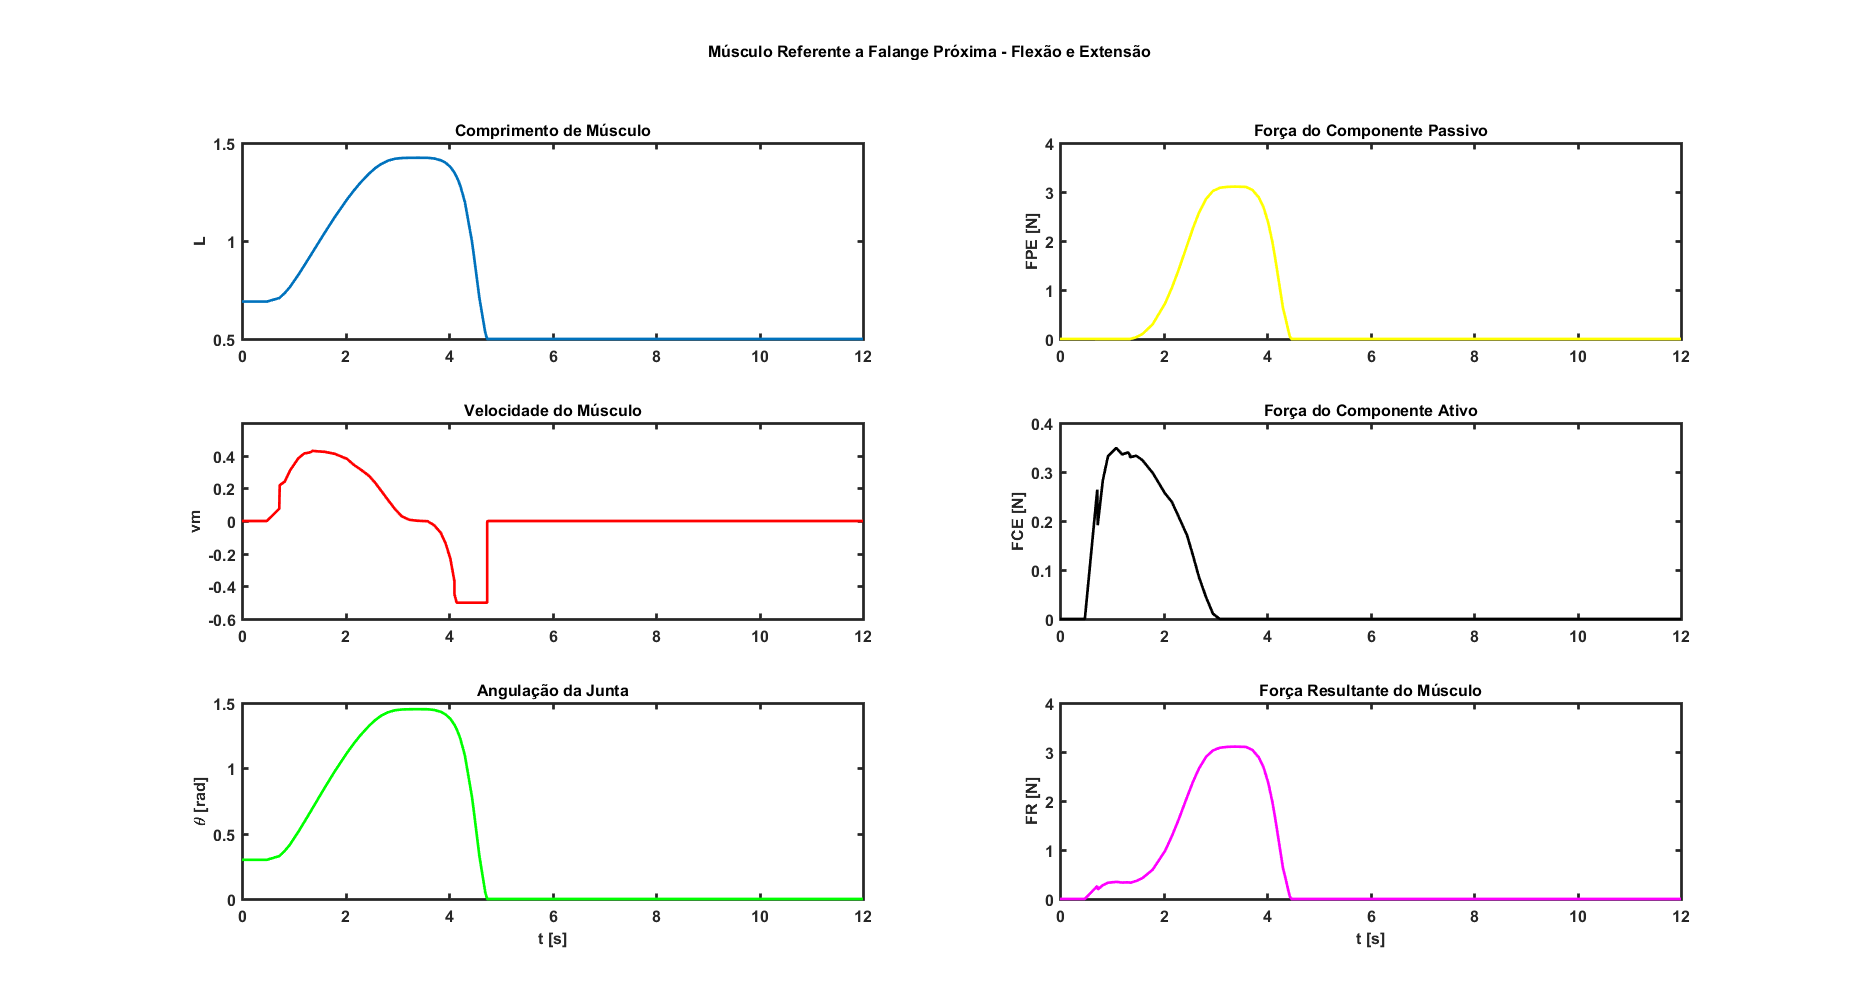
\includegraphics[width = 1\textwidth]{img/flexao_extensao.png}
\caption[Resposta ao Movimento de Flexão e em seguida Extensão para uma Falange Próxima]{Resposta ao Movimento de Flexão e em seguida Extensão para uma Falange Próxima}
\label{sim_flexao_extensao}
\end{figure}

Logo nota-se que, primeiramente o elemento CE responde diretamente ao nível de atuação, e a medida que o comprimento do músculo varia o elemento PE responde com uma força proporcional. Os maiores valores de $\theta$ são acompanhados do aumento da velocidade e normalmente ocorrem logo após estes, o que demonstra uma robustez física do modelo, assim como o fato de os movimentos opostos resultarem em um comprimento final tendendo a 0 para o músculo. 

Com um movimento completo de flexão e extensão, é possível correlacionar as curvas de ângulo da junta e velocidade com as obtidas por \cite{rosen1999performances}, demonstradas na figura \ref{rosen_ativacao}. Lembra-se que o estudo performado por \cite{rosen1999performances} se tratava de uma captura de dados utilizando a tecnologia sEMG, a qual possui ruídos, os quais não existem nestas simulações, já que foram feitas utilizando curvas ideais produzidas pelo \textit{MATLAB}.

\begin{figure}[H]
\centering
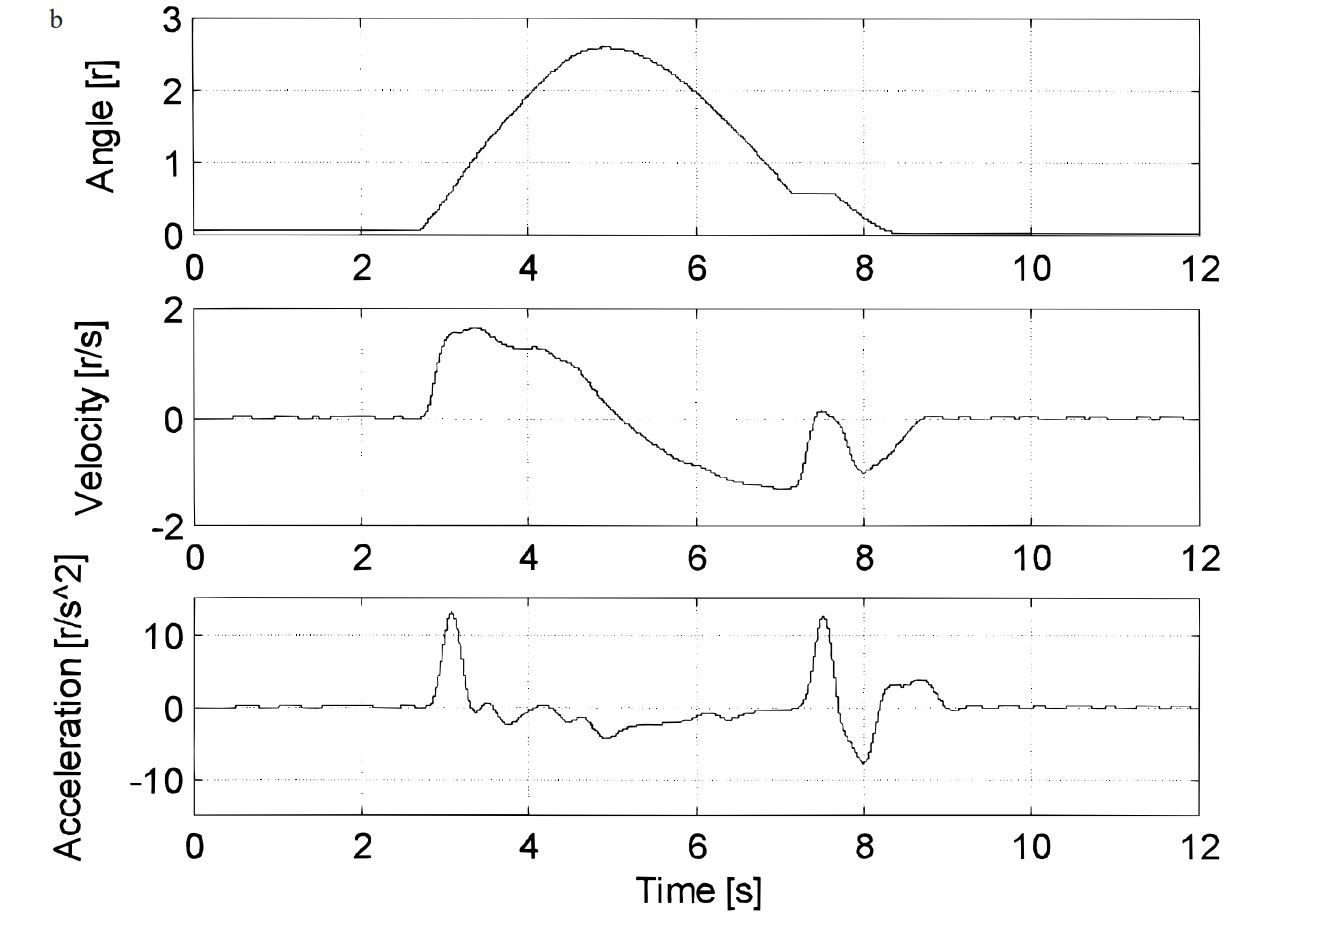
\includegraphics[width = 1\textwidth]{img/Rosen1999_ativacao.JPG}
\caption[Resposta ao Movimento de Flexão seguido de Extensão em um Ombro]{Registros de uma sessão típica. Cinemática do ombro : ângulo da articulação do ombro, velocidade angular, e aceleração angular \cite{rosen1999performances}}
\label{rosen_ativacao}
\end{figure}

\section{Simulação do Movimento}
\label{resultado_simulacao}
Para uma validação do modelo completo é necessário que se faça a composição das duas validações anteriores, sendo assim nesta seção foi feita a simulação dos dedos da mão humana levando em consideração inputs como os da seção \ref{resultado_ativacao}. O modelo desenvolvido neste projeto é normalizado, portanto aqui pode-se simular o dedo polegar e os outros dedos da mão sem perder a coerência das validações. Sabendo disso, nesta seção é feita a simulação parcial do dedo, onde apenas uma junta é estimulada (descrita na tabela \ref{tabela_seq_uma} e a simulação completa do dedo onde é feita então a simulação de duas sequências de movimentos compostas por movimentos de flexão e extensão como previsto na seção \ref{integracao_validacao}, as duas sequências estão demonstradas na tabela \ref{tabela_sequencia_movimentos}.

\begin{table}[H]
\centering
\caption{Tabela das Sequências de Movimentos para uma Junta}
\label{tabela_seq_uma}
\begin{tabular}{|c|c|}
	\hline
    \# & Sequência \\ \hline
    1 & $f_{PIP} -> e_{PIP}$ \\ \hline
\end{tabular}
\end{table}

\begin{table}[H]
\centering
\caption{Tabela das Sequências de Movimentos para Todas as Juntas}
\label{tabela_sequencia_movimentos}
\begin{tabular}{|c|c|}
	\hline
    \# & Sequência \\ \hline
    1 & $f_{PIP} -> e_{PIP} -> f_{MP_{F}} -> e_{MP_{F}} -> f_{MP_{AA}} -> e_{MP_{AA}}$  \\ \hline
    2 & $f_{PIP} -> f_{MP_{F}} -> f_{MP_{AA}} -> e_{PIP} -> e_{MP_{F}} -> e_{MP_{AA}}$ \\ \hline
\end{tabular}
\end{table}

Onde $f_{x_y}$ é o movimento de flexão do músculo relativo a junta x no músculo responsável por y da junta, por exemplo $f_{MP_{AA}}$ é o movimento de flexão da junta MP em movimento de adução/abdução.

\subsection{Movimento de uma Junta}
A primeira validação é feita em cima da movimentação de apenas uma junta, pela sequência determinada na tabela \ref{tabela_seq_uma}. Para simplificação e coerência com o resto das análises feitas no projeto, esta validação foi feita em cima do dedo anelar. Então, para a movimentação de apenas uma junta foi utilizado como input do modelo de ativação muscular os níveis de atuação descritos na figura \ref{ativacao_musculos}. Os resultados do modelo de ativação muscular (os ângulos das articulações) alimentam o modelo de cinemática direta da mão, como proposto em \ref{simulacao_mao}. Estes foram utilizados para movimentar a articulação PIP, pois, por motivos visuais e experimentais ela é a melhor articulação para mostrar os resultados do modelo. Como a articulação DIP se move em função da PIP, fica visível a relação entre os movimentos. A movimentação do dedo anelar para a entrada da figura \ref{ativacao_musculos} está descrita na figura \ref{movimentacao_uma_junta}.

\begin{figure}[H]
\centering
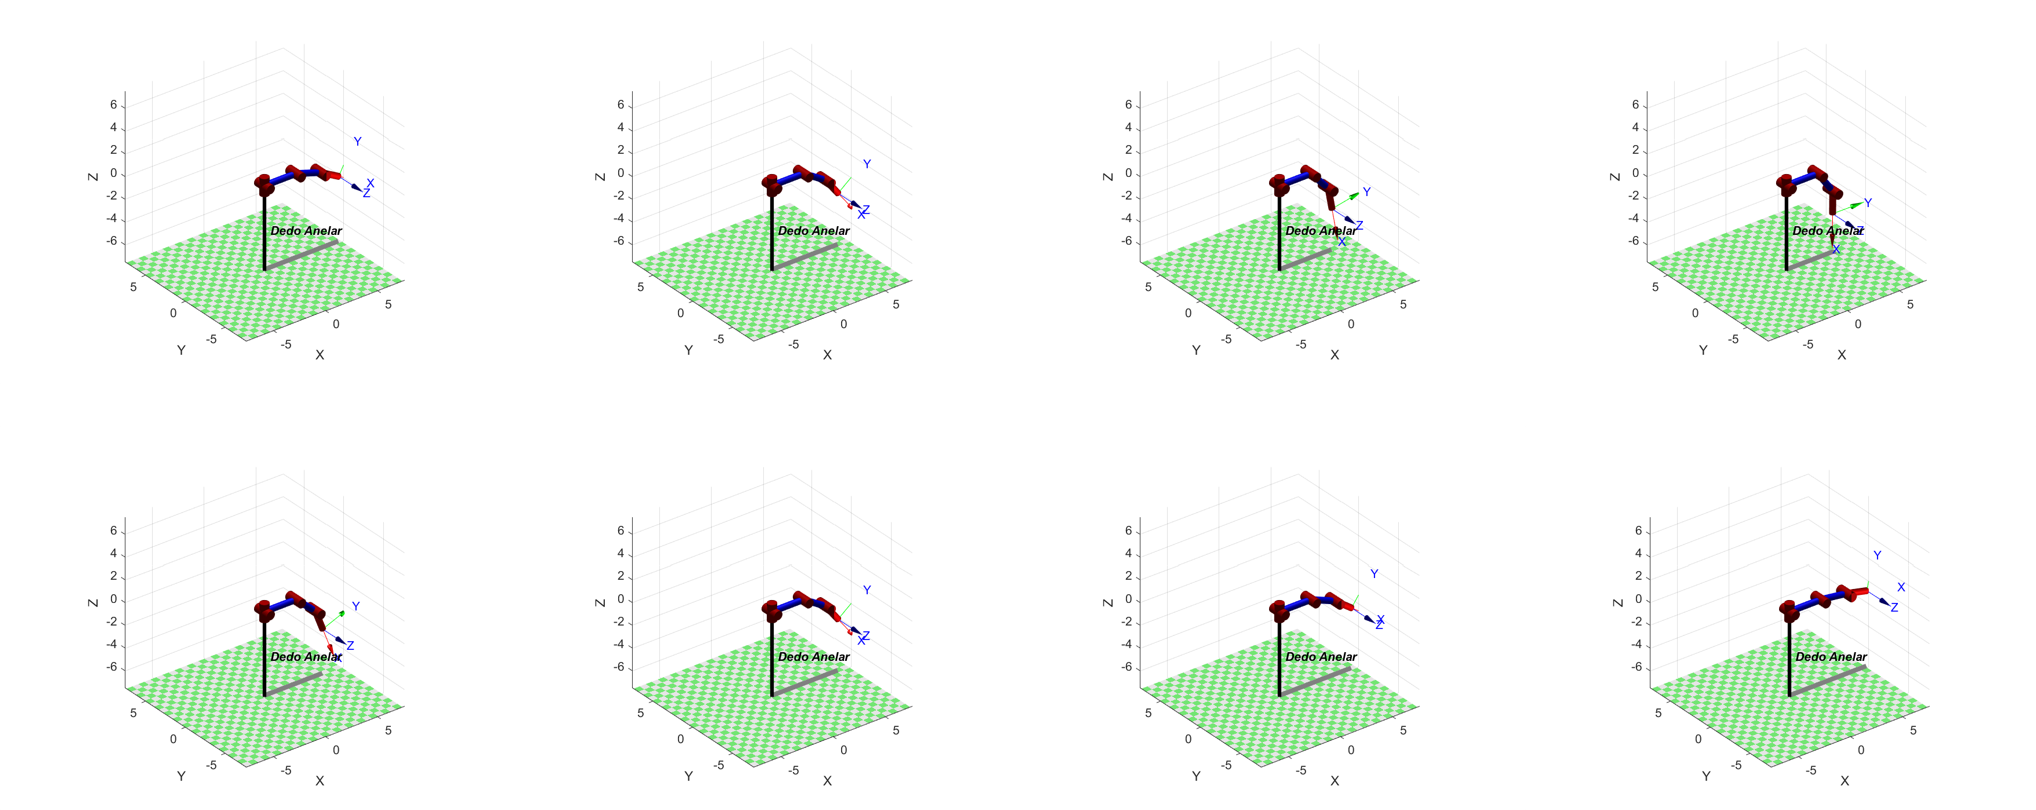
\includegraphics[width = 1\textwidth]{img/sim_uma_junta.png}
\caption[Simulação do Movimento de uma Junta]{Simulação do Movimento de uma Junta}
\label{movimentacao_uma_junta}
\end{figure}

É possível notar na linha de cima da figura \ref{movimentacao_uma_junta} o movimento de flexão da junta PIP, que por consequência também movimenta a junta DIP, e na linha de baixo está o movimento de extensão da junta PIP.

\subsection{Movimento Completo}
Como descrito na tabela \ref{tabela_sequencia_movimentos}, para a validação do movimento completo irão ser feitas duas sequências de movimentos envolvendo todos os músculos do dedo anelar modelado neste projeto.

Para a primeira simulação, a fim de executar a sequência 1, foram destacados os seguintes níveis de ativação, descritos na figura \ref{niveis_atuacao_simulacao}. Primeiramente é feito uma sequência de flexão e extensão nos músculos da junta PIP, e então uma sequência de flexão e extensão nos músculos da junta MP em movimento de flexão, e finalmente uma sequência de flexão e extensão nos músculos da junta MP em movimento de adução/abdução.

\begin{figure}[H]
\centering
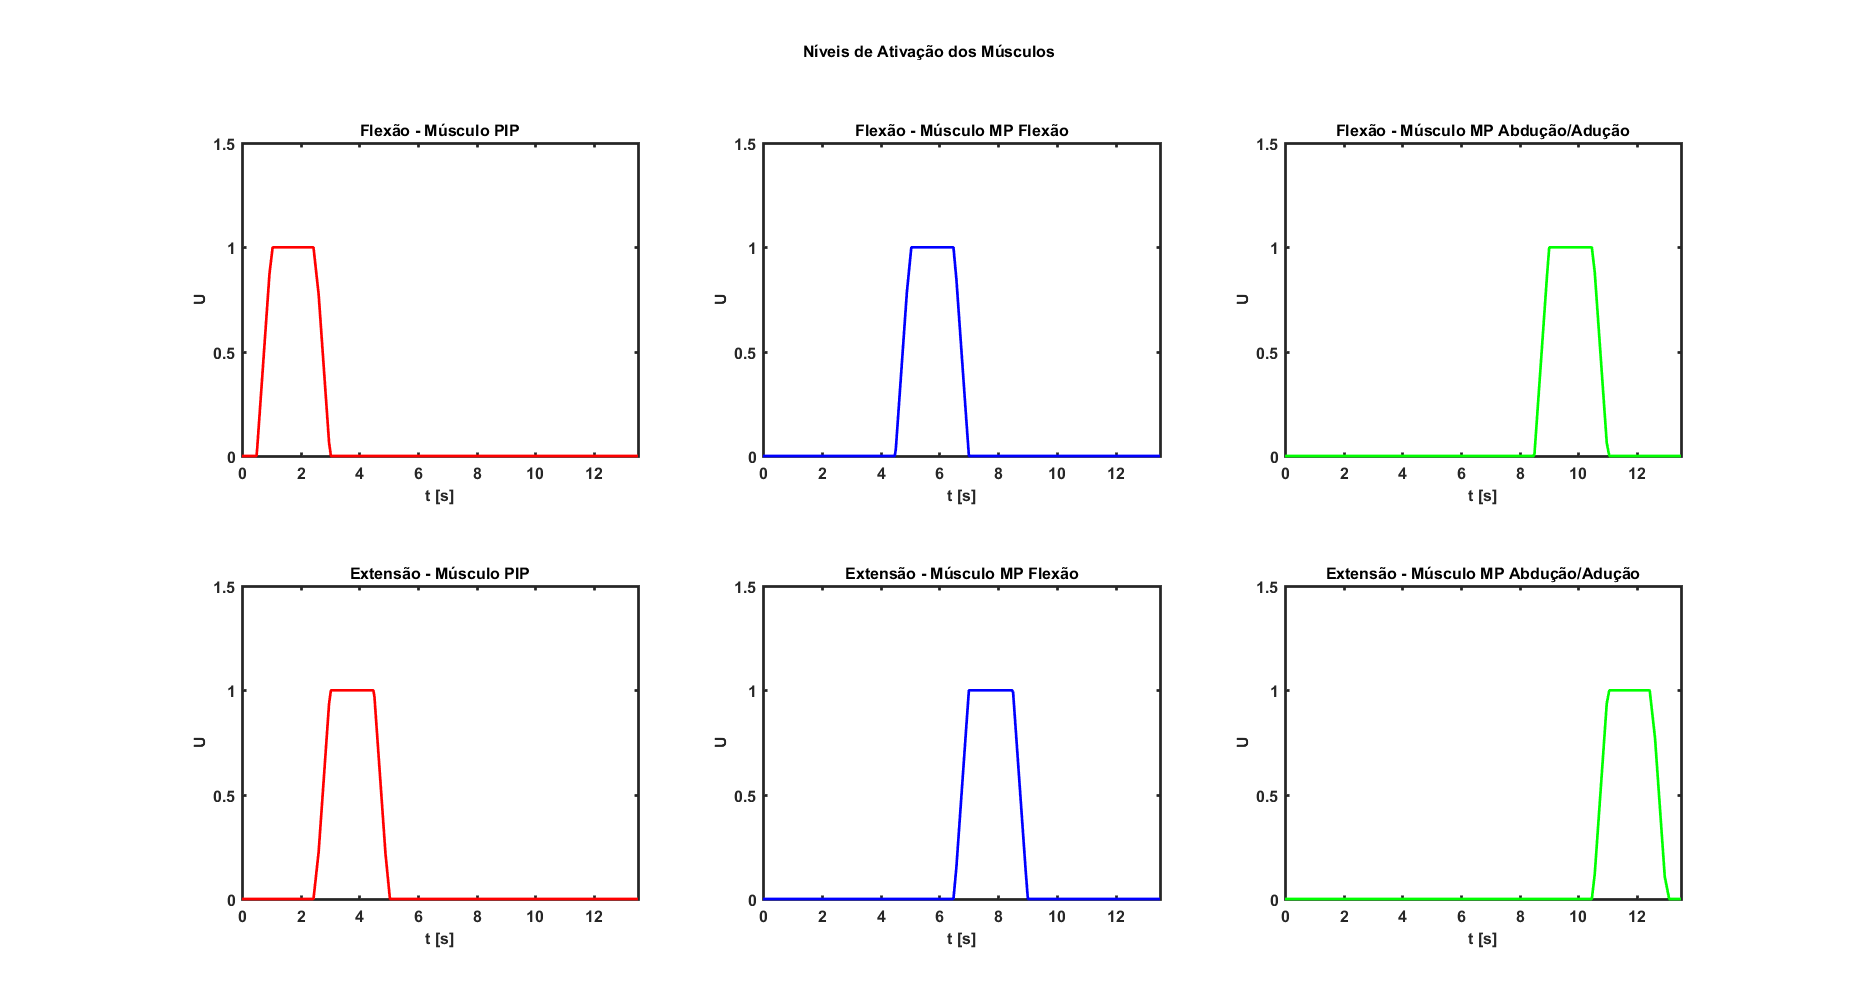
\includegraphics[width = 1\textwidth]{img/niveis_simulacao.png}
\caption[Níveis de Atuação Utilizados em cada Músculo na Simulação Completa do Movimento do Dedo Anelar para a Sequência 1]{Níveis de Atuação Utilizados em cada Músculo na Simulação Completa do Movimento do Dedo Anelar para a Sequência 1}
\label{niveis_atuacao_simulacao}
\end{figure}

Na figura \ref{simulacao_sequencia_1}, é possível notar a sequência de movimentos determinada pela sequência 1. Um músculo flexiona e extende, e então o próximo músculo dá continuidade no movimento fazendo a mesma repetição. Lembra-se que a amplitude dos movimentos é diferente pois, conforme as restrições descritas em \ref{anatomia_mao} e o MJG de cada falange, o range de atuação de cada articulação é diferente.

\begin{figure}[H]
\centering
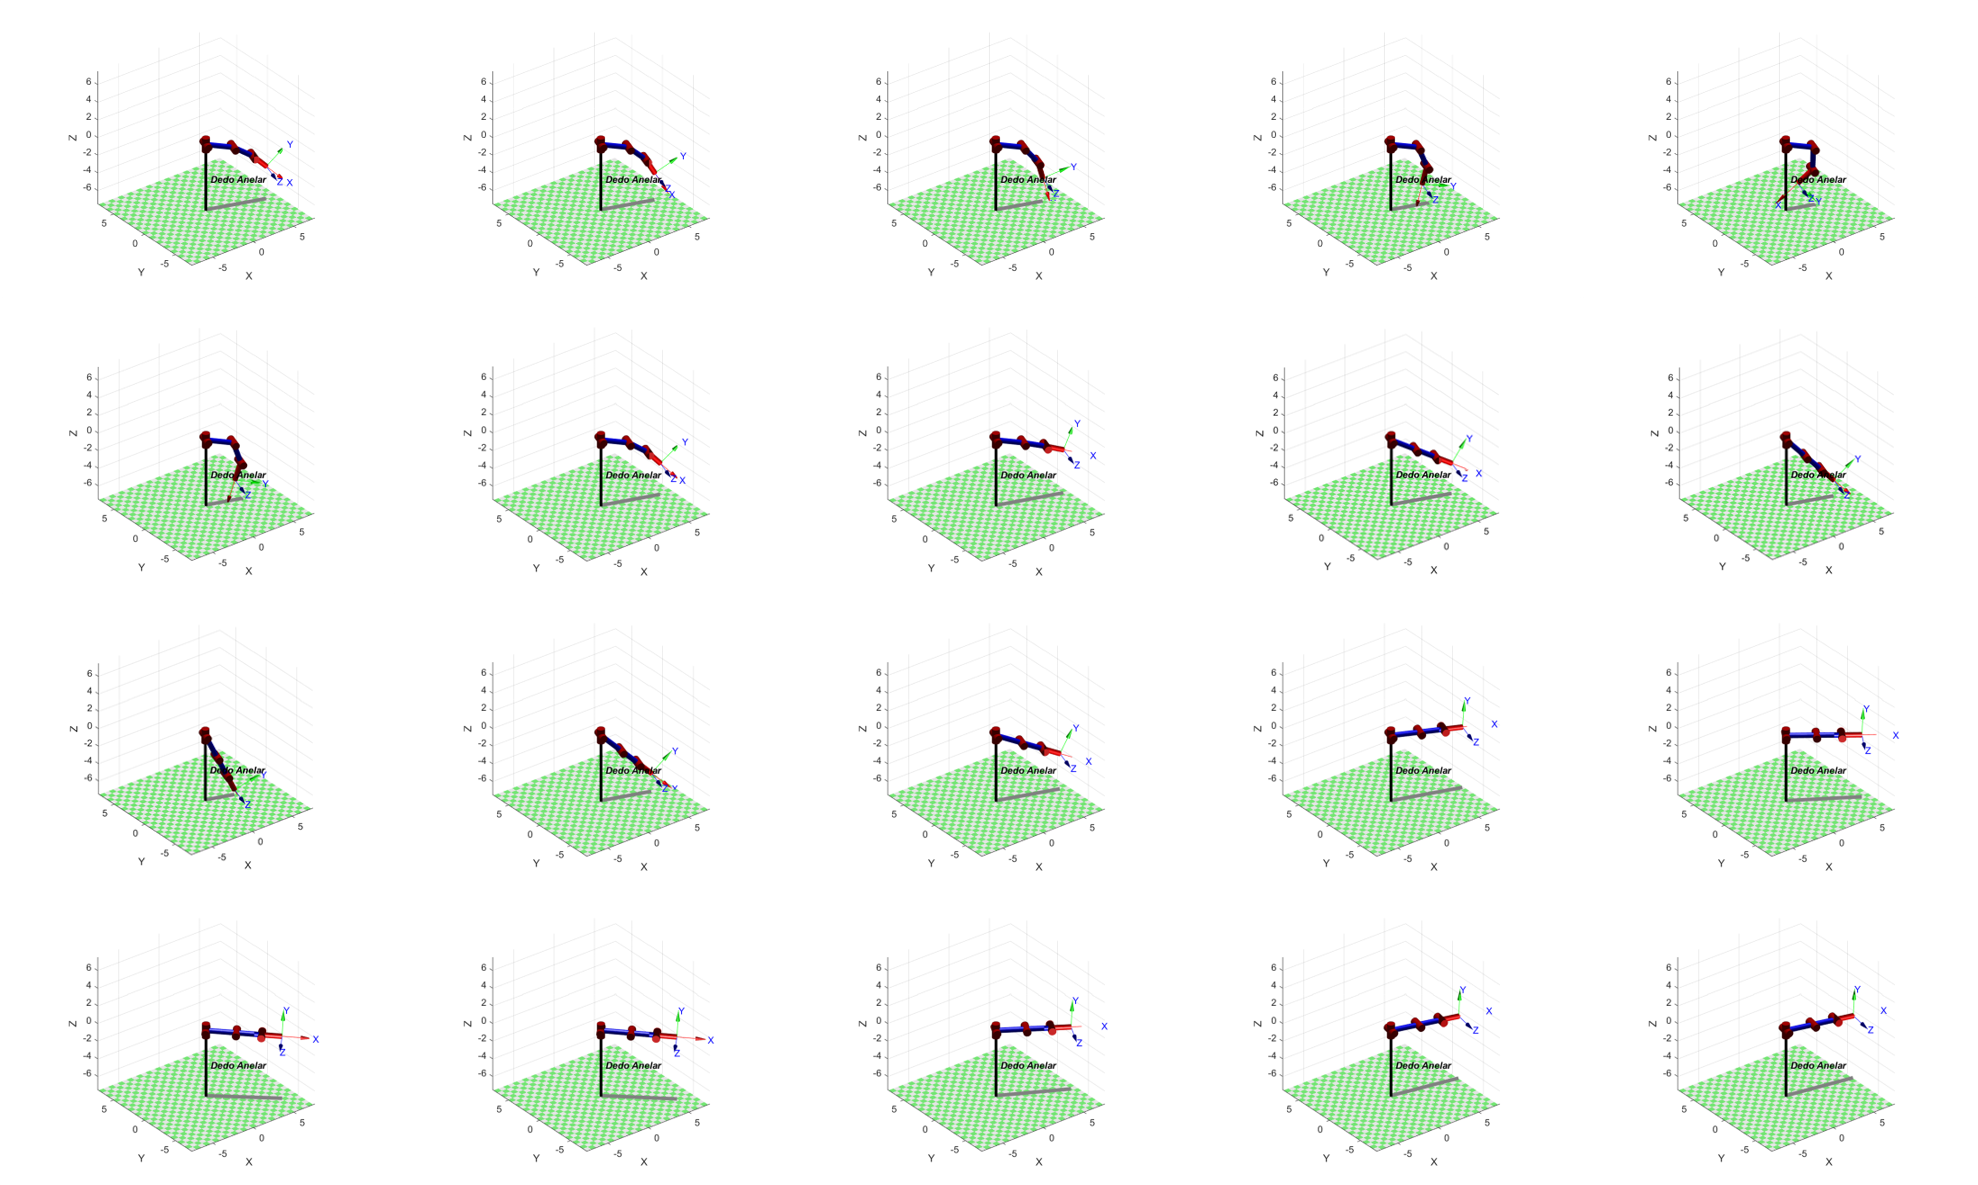
\includegraphics[width = 1\textwidth]{img/simulacao_sequencia_1.png}
\caption[Sequência 1 de Movimentos para o Dedo Anelar]{Sequência 1 de Movimentos para o Dedo Anelar}
\label{simulacao_sequencia_1}
\end{figure}

Para a segunda simulação, a fim de executar a sequência 2, foram destacados os níveis de atuação descritos na figura \ref{niveis_atuacao_simulacao2}. Nesta simulação a sequência de movimento consiste em fazer o movimento de flexão em todos os músculos e então o movimento de extensão em todos eles, seguindo a ordem de músculos: PIP, MP flexão e MP adução/abdução.

\begin{figure}[H]
\centering
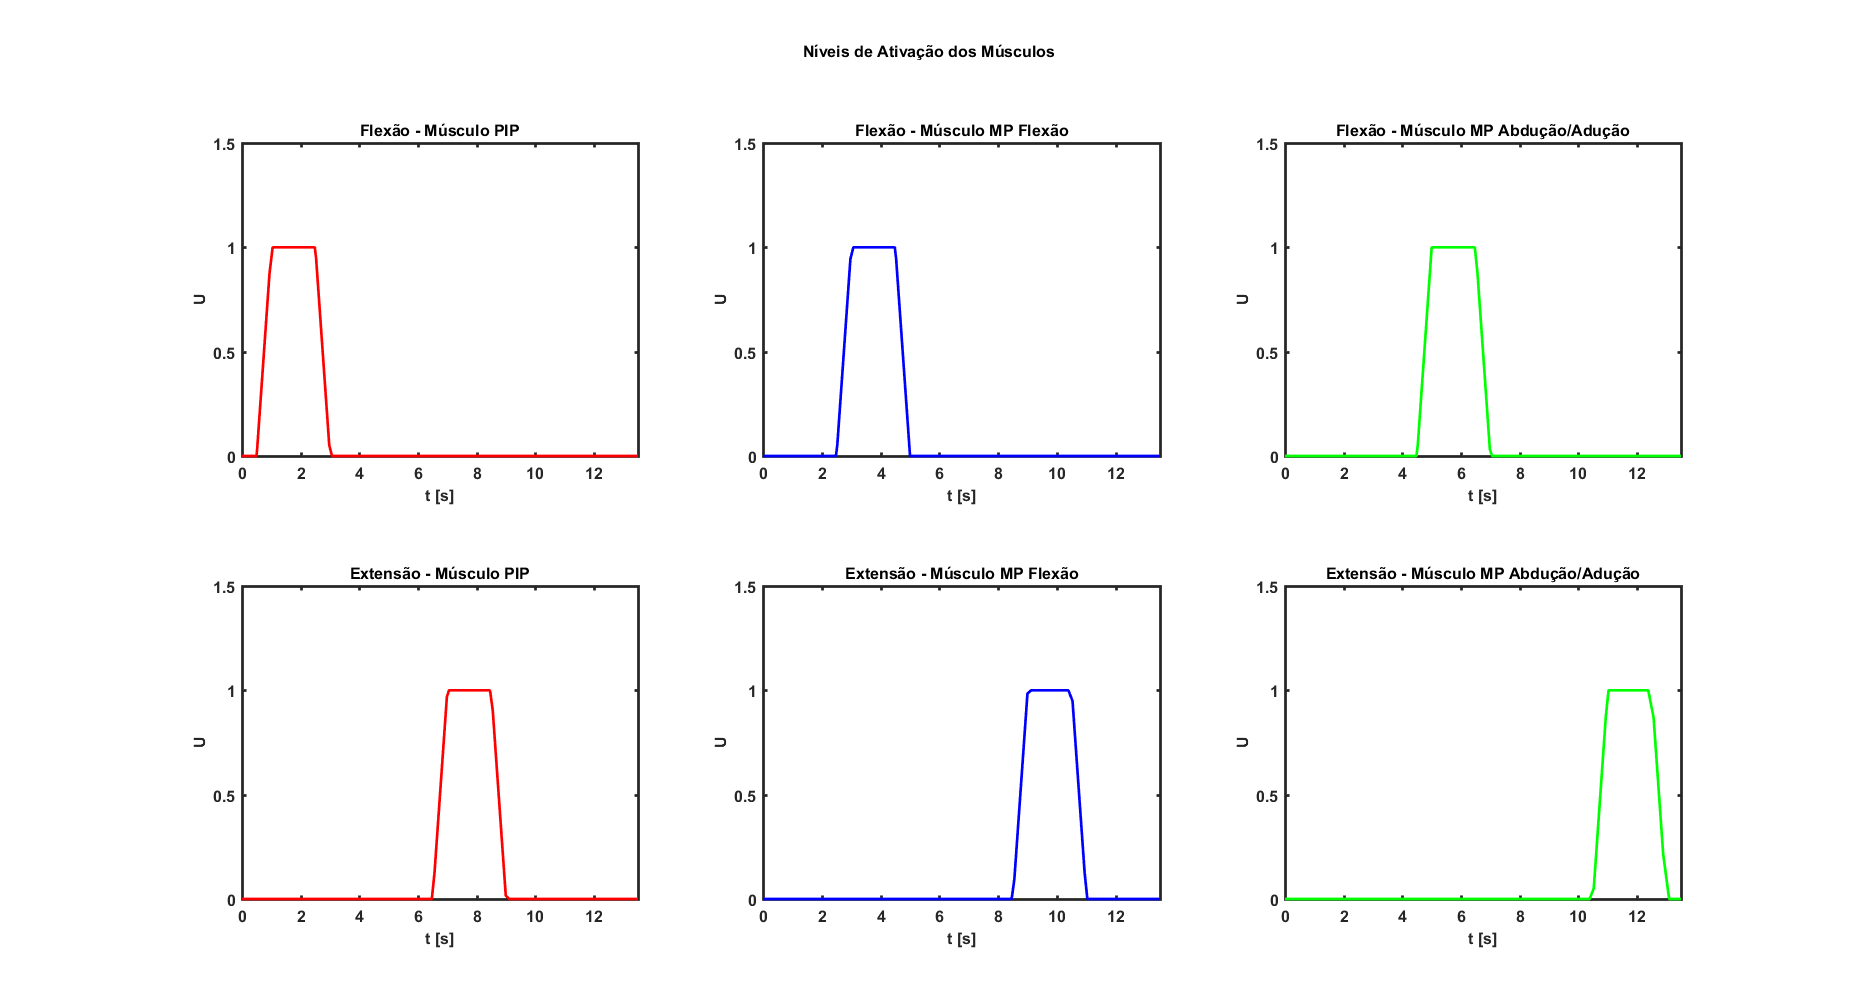
\includegraphics[width = 1\textwidth]{img/niveis_simulacao2.png}
\caption[Níveis de Atuação Utilizados em cada Músculo na Simulação Completa do Movimento do Dedo Anelar para a Sequência 2]{Níveis de Atuação Utilizados em cada Músculo na Simulação Completa do Movimento do Dedo Anelar para a Sequência 2}
\label{niveis_atuacao_simulacao2}
\end{figure}

Na figura \ref{simulacao_sequencia_2}, é possível notar o comportamento dos músculos. Mesmo alterando a sequência eles continuam agindo conforme o esperado. Os ângulos das juntas PIP e DIP se movem em conjunto e nesta sequência de movimentos a ponta do dedo chega mais perto do que seria representado como a palma da mão. Isto demonstra como diferentes sequências de movimentos podem fazer o dedo atingir posições distintas e distâncias diferentes em relação ao eixo principal.

\begin{figure}[H]
\centering
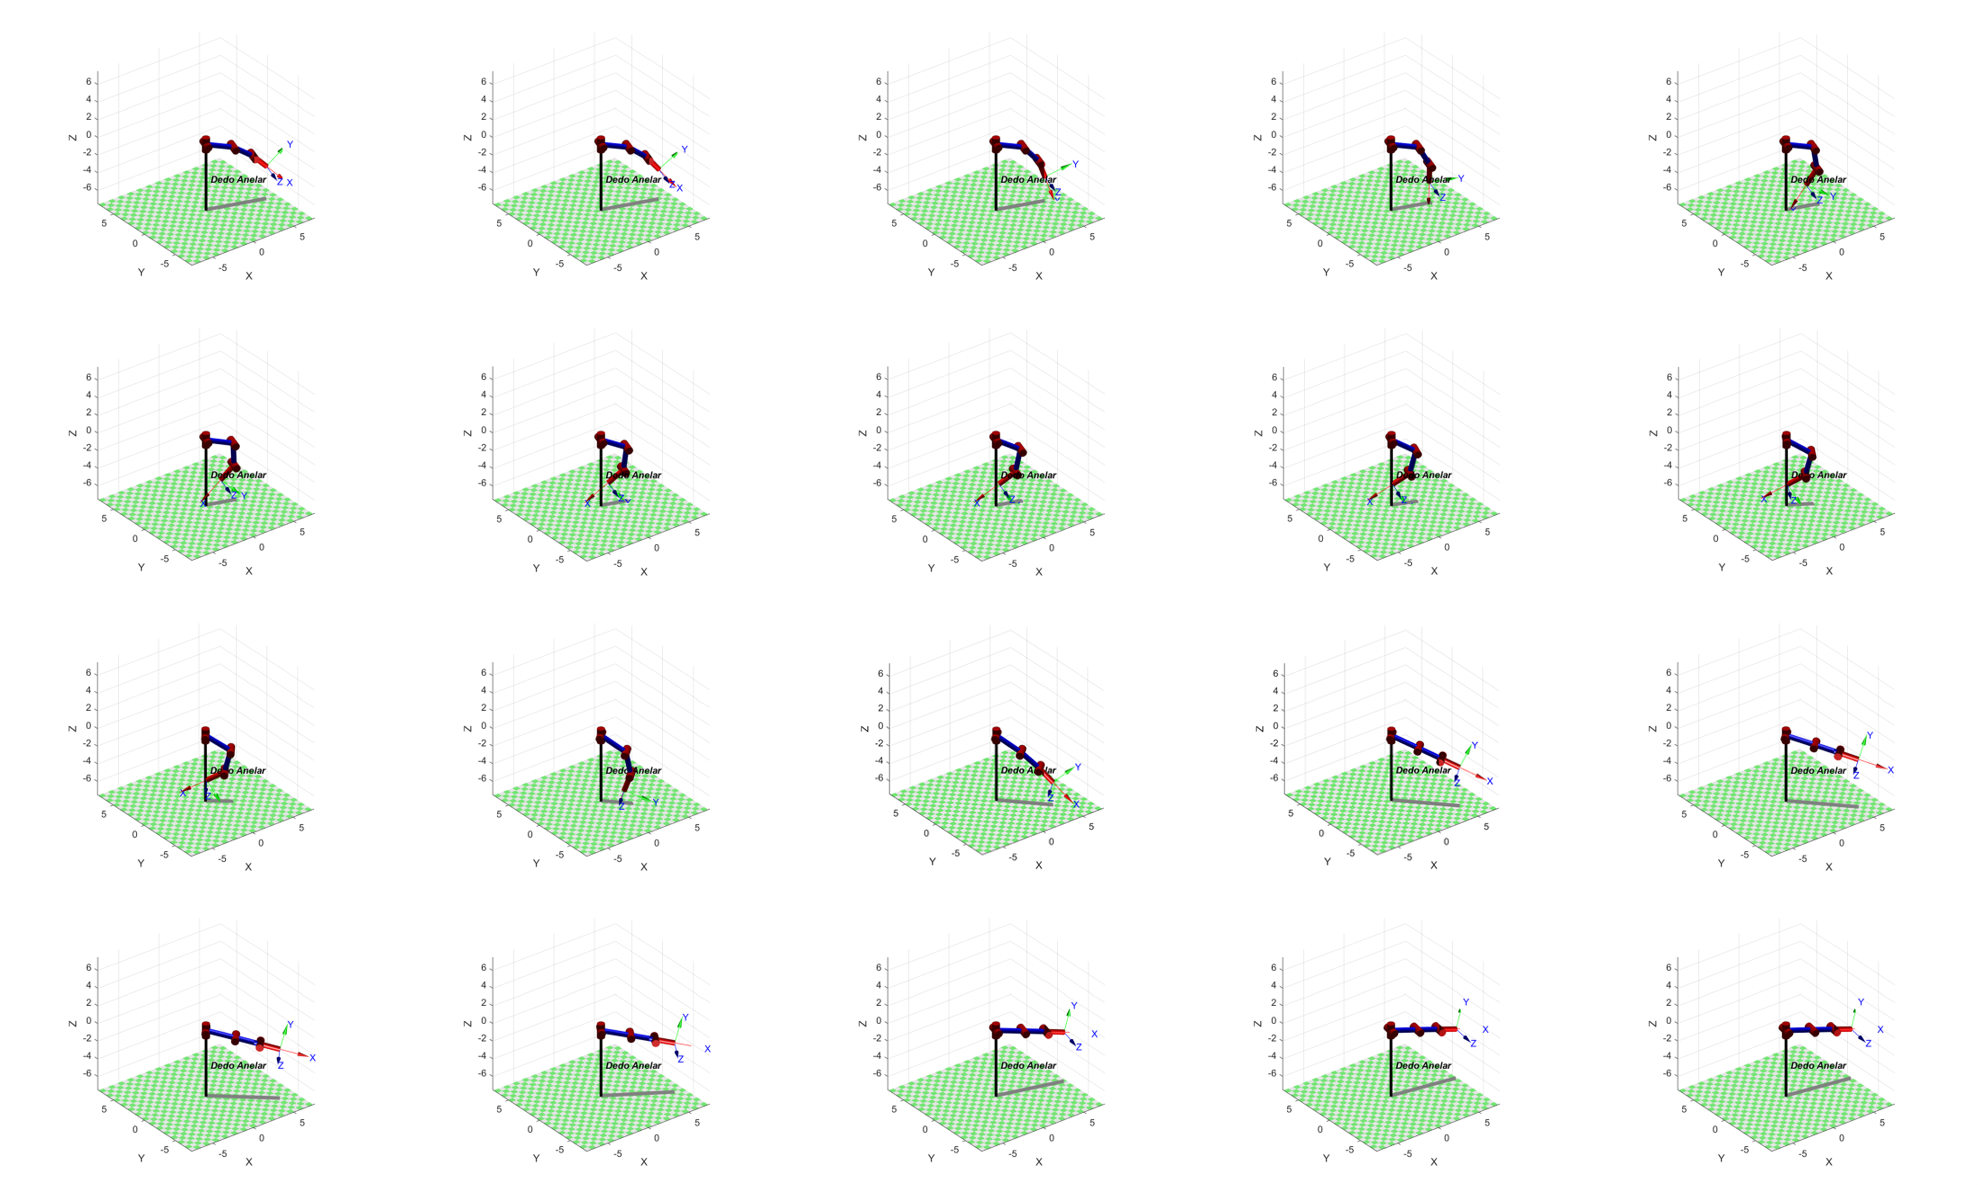
\includegraphics[width = 1\textwidth]{img/simulacao_sequencia_2.png}
\caption[Sequência 2 de Movimentos para o Dedo Anelar]{Sequência 2 de Movimentos para o Dedo Anelar}
\label{simulacao_sequencia_2}
\end{figure}